
\documentclass[a4paper,11pt]{report}

\usepackage[utf8]{inputenc}
\usepackage[T1]{fontenc}
\usepackage{amsmath}
\usepackage{amssymb,calc}
\usepackage[francais]{babel}

\usepackage{cases}

\usepackage{wrapfig}

\usepackage[colorlinks=false]{hyperref}

% Pour se passer du préfixe FIGURE
\usepackage[labelformat=empty]{caption}

% Pour les matrices annotées ... 
\usepackage{blkarray}

% Pour les figures
\usepackage{graphicx}

% Pour les listes à puces
\usepackage{enumitem}

\usepackage{indentfirst}

% Pour splitter une page
\usepackage{multicol}


% Évite un conflit entre french babel et enumitem
\frenchbsetup{StandardLists=true}

\usepackage[standard,framed]{ntheorem}
\usepackage{framed}

% Pour les matrices par blocs je crois ?
\makeatletter
\renewcommand*\env@matrix[1][*\c@MaxMatrixCols c]{%
  \hskip -\arraycolsep
  \let\@ifnextchar\new@ifnextchar
  \array{#1}}
\makeatother

% Pour annoter les matrices :
%\usepackage{kbordermatrix} 
%\renewcommand{\kbldelim}{(} % change default array delimiters to parentheses
%\renewcommand{\kbrdelim}{)}


% Pour des matrices agrandies :
\newenvironment{bigmatrix}[2]{%
  \renewcommand*{\arraystretch}{#1}% 
  \begin{pmatrix}[#2]
}{%
  \end{pmatrix}
}

% Pour des commentaires à droite d'équations
\newenvironment{rcases}
  {\left.\begin{aligned}}
  {\end{aligned}\right\rbrace}

\newenvironment{lcases}
  {\left\lbrace\begin{aligned}}
  {\end{aligned}\right.}


\setlength{\parindent}{30pt}
\setlength{\parskip}{1ex}
\setlength{\textwidth}{15cm}
\setlength{\textheight}{24cm}
\setlength{\oddsidemargin}{0.2cm}
\setlength{\evensidemargin}{-.7cm}
\setlength{\topmargin}{-.5in}

% Commandes pour les maths :
\newcommand{\reff}[1]{(\ref{#1})}
\newcommand{\dx}{\,dx}
\newcommand{\dt}{\,dt}
\newcommand{\ito}{,\dotsc,}
\newcommand{\R}{\mathbb{R}}
\newcommand{\N}{\mathbb{N}}
\newcommand{\C}{\mathbb{C}}
\newcommand{\Z}{\mathbb{Z}}
\newcommand{\gO}{\mathcal{O}}
\newcommand{\Poly}[1]{\mathcal{P}_{#1}}
\newcommand{\abs}[1]{\left\lvert#1\right\rvert}
\newcommand{\norm}[1]{\left\lVert#1\right\rVert}
\newcommand{\pars}[1]{\left(#1\right)}
\newcommand{\bigpars}[1]{\bigl(#1\bigr)}
\newcommand{\set}[1]{\left\{#1\right\}}
\newcommand{\tpo}[1]{\,^t#1}
\newcommand{\derpart}[2]{\displaystyle\frac{\partial#1}{\partial #2}}
\newcommand{\der}[2]{\displaystyle\frac{\text{d}#1}{\text{d} #2}}
\newcommand{\deffonc}[3]{#1 : #2 \longrightarrow #3}
\newcommand{\Co}{\mathcal{C}}
\newcommand{\MinI}[1]{\underset{#1}{\text{Min }}}
\newcommand{\MaxI}[1]{\underset{#1}{\text{Max }}}

\DeclareMathOperator{\Sup}{Sup}
\DeclareMathOperator{\Max}{Max}
\DeclareMathOperator{\Det}{Det}
\DeclareMathOperator{\diag}{diag}
\DeclareMathOperator{\Min}{Min}
\DeclareMathOperator{\Inf}{Inf}

% Je ne sais plus pourquoi ??
\newlength\dlf
\newcommand\alignedbox[2]{
  % #1 = before alignment
  % #2 = after alignment
    &
    \begingroup
    \settowidth\dlf{$\displaystyle #1$}
    \addtolength\dlf{\fboxsep+\fboxrule}
    \hspace{-\dlf}
    \boxed{#1 #2}
\endgroup
}

%%%%% PACKAGE AMSTHM :
% \newtheoremstyle{definition}
%   {20pt}   % ABOVESPACE
%   {20pt}   % BELOWSPACE
%   {}  % BODYFONT
%   {0pt}       % INDENT (empty value is the same as 0pt)
%   {\bfseries} % HEADFONT
%   {.}         % HEADPUNCT
%   {5pt plus 1pt minus 1pt} % HEADSPACE
%   {}          % CUSTOM-HEAD-SPEC

\newframedtheorem{ftheo}[theorem]{Théorème}

\theoremstyle{plain} % default
\theorembodyfont{\normalfont}
\newframedtheorem{fdef}[definition]{Définition}

\renewtheorem{remark}{Remarque}

\newframedtheorem{coroll}{Corollaire}

\newframedtheorem{prop}{Proposition}

\newtheorem{rappel}{Rappel}
\newtheorem{preuve}{Preuve}
\newtheorem{exemple}{Exemple}
\newframedtheorem{lemme}{Lemme}



%%%%%%%%%%%%%%%% PAGE DE GARDE %%%%%%%%%%%%%%%%%%%%%%
% Crédit : http://www.grappa.univ-lille3.fr/FAQ-LaTeX/6.67.html
\newlength{\larg}
\setlength{\larg}{14.5cm}

\title{
{\rule{\larg}{1mm}}\vspace{7mm}
\begin{tabular}{p{2cm} r}
   & {\Huge {\bf Méthodes numériques de base}} \\
   & \\
   & {\huge Cours de première année - ENSIMAG}
\end{tabular}\\
\vspace{2mm}
{\rule{\larg}{1mm}}
\vspace{2mm} \\
\begin{tabular}{p{11cm} r}
   & {\large \bf } \\
   & {\large }
\end{tabular}\\
\vspace{5.5cm}
}
\author{\begin{tabular}{p{13.7cm}}
    \begin{tabular}{ll}
        Cours : & Hahmann S.\\
         & James G.\\
    \LaTeX : & Poupin P.
    \end{tabular}
\end{tabular}\\
\hline }
\date{}

%%%%%%%%%%%%%%%%%%%%%%%%%%%%%%%%%%%%%%

% \includeonly{methodes_num6}

\pagestyle{headings}

\begin{document}

\maketitle

\tableofcontents

\chapter{Approximation de problèmes aux limites par différences finies}

\section{Introduction}

On considère ici des problèmes aux limites en une dimension,
linéaires, du second ordre :

\begin{subnumcases}{}
- u''(x) + p(x) u'(x) + q(x) u(x) = f(x) \hspace{1cm} x \in ]a,b[ \label{eq:1-pbvp-1}\\
    \left.\begin{array}{c}
        u(a) = \alpha \\
        u(b) = \beta
    \end{array} \right\rbrace \label{eq:1-pbvp-cl}
\end{subnumcases}
où $p,q,f \in \Co^0([a,b])$ et $\alpha,\beta \in R$. On a une équation
différentielle linéaire du 2\up{nd} ordre, à coefficients a priori variables,
augmentée des conditions aux limites \eqref{eq:1-pbvp-cl}.
Ces conditions fixent la valeur de $u$ au bord du domaine : on parle de
\textbf{conditions de Dirichlet}.

Lorsque les conditions aux limites fixent la valeur de $u'$ au bord 
($u'(a)=\alpha,u'(b)=\beta$), on parle de conditions de \textbf{Neumann}.

\subsection*{Exemples issus de la physique}
\begin{enumerate}[label=\alph*)]
    \item 
        \[
            \left\lbrace
            \begin{array}{lll}
                \dfrac{d^2\phi}{dr^2} + \dfrac{1}{r} \dfrac{d\phi}{dr} = \lambda \phi & , & r \in ]r_a,R[
                    \\ [5pt]
            \phi'(r_a) = \alpha
            \\ [2pt]
            \phi'(R) = 0
            \end{array}
            \right.
        \]

        Equations de Debye-Hückel donnant le potentiel électrique $\phi$ autour
        d'un cylindre chargé (de rayon $r_a$) polongé dans une solution
        ionique ($r_a < r < R$).

    \item 
        \[
            \left\lbrace
            \begin{array}{lll}
            - \dfrac{d}{dx}\left( k(x) \dfrac{du}{dx} \right) = f(x) & , & x \in ]0,L[
            \\ [5pt]
            u(0) = 0
            \\ [2pt]
            u(L) = 0 
            \end{array}
            \right.
        \]

        Equation de la chaleur stationnaire donnant la température $u$ dans
        une barre de longueur $L$ chauffée et de conductivité $k(x)$ variable.
        ($f(x) = $ quantité de chaleur fournie par unité de temps et de longueur).
        La température aux extrémités de la barre est maintenue à 0.
\end{enumerate}

Lorsque $q \geq 0$, le résultat suivant assure que \eqref{eq:1-pbvp-1} - \eqref{eq:1-pbvp-cl}
possède une solution unique. Mais on n'a pas en général d'expression explicite
de $u$ quand $p$ ou $q$ dépendent de $x$.

\begin{ftheo}
    Si $q(x) \geq 0$ sur $[a,b]$ alors \eqref{eq:1-pbvp-1} - \eqref{eq:1-pbvp-cl}
    \textbf{admet une unique solution} $u \in \Co^2([a,b])$.
    
    De plus, si $p,q,f \in \Co^k([a,b])$
    alors $\boxed{u \in \Co^{k+2}([a,b])}$.
\end{ftheo}

\begin{preuve}[de l'unicité]
    Si $u_1$ et $u_2$ vérifient \eqref{eq:1-pbvp-1} - \eqref{eq:1-pbvp-cl}, alors
    $v = u_1 - u_2$ est solution du problème homogène :
    \[
        \left\lbrace
        \begin{array}{l}
            -v'' + pv' + qv = 0 \\
            v(a) = v(b) = 0
        \end{array}
        \right.
    \]

    Notons $r(x) = e^{-\int p \dx}$ et $s(x) = q(x) e^{-\int p \dx}$.
    En multipliant l'équation par $r$ on a :
    \[
       -\left( r(x) v'(x) \right)' + s(x) v(x) = 0
    \]

    On multiplie maintenant cette équation par $v$ et on intègre sur $[a,b]$,
    en utilisant les conditions aux limites :

    \[
        \int_a^b r (x) v'^2 \dx + \int_a^b s(x) v^2 \dx = 0
    \]
    avec $r>0$ et $s \geq 0$

    Donc $\int_a^b r(x) v'^2 \dx = 0 \implies v'=0$ (puisque $r>0$) $\implies v = 0$ à cause des conditions aux limites.
\end{preuve}

L'existence d'une solution $u \in \Co^2([0,1])$ peut être obtenue de différentes façons
(méthode de variation de la constante, méthodes d'analyse fonctionnelle,
par exemple formulation variationnelle).
La régularité $\Co^k$ de $u$ s'obtient simplement par récurrence sur $k$.

\section{Discrétisation par différences finies}

Nous allons étudier comment calculer $u$ numériquement.

\[
    (p) \;
    \left\lbrace
    \begin{array}{cc|c}
        -u'' + p(x) u' + q(x) u = f(x) &  & x \in ]a,b[ \\
            u(a) = \alpha &  & p,q,f \in \Co^0([a,b]) \\
            u(b) = \beta &  & q \geq 0 \text{ sur } [a,b]
    \end{array}
    \right.
\]

On discrétise $[a,b]$ suivant les points $x_i = a + ih$ ($i=0,\dots,N+1$)
avec $h = \frac{b-a}{N+1}$. On notera $u_i$ la valeur approchée de
$u(x_i)$ à calculer et $U = \tpo (u_1, \dots, u_N)$, $(u_0 = \alpha, u_{N+1} = \beta)$.

On approche $u''(x_i)$ et $u'(x_i)$ en utilisant un développement de Taylor
de $u$ en $x_i$.

Si $u \in \Co^4([a,b])$ :
\[
    u(x_{i+1}) = u(x_i + h) = u(x_i) + h \: u'(x_i) + \frac{h^2}{2} u''(x_i)
    + \frac{h^3}{6} u^{(3)}(x_i) + \frac{h^4}{24} u^{(4)}(\theta_i^+)
\]
\hfill avec $\theta_i^+ \in ]x_i,x_{i+1}[$

\[
    u(x_{i-1}) = u(x_i + h) = u(x_i) - h \: u'(x_i) + \frac{h^2}{2} u''(x_i)
    - \frac{h^3}{6} u^{(3)}(x_i) + \frac{h^4}{24} u^{(4)}(\theta_i^-)
\]
\hfill avec $\theta_i^- \in ]x_{i-1},x_i[$

    Donc :
    \[
        \frac{u(x_{i+1}) - u(x_{i-1})}{2h} =  u'(x_i) + \mathcal{O}(h^2)
    \]
    \[
        \frac{u(x_{i+1}) - u(x_i) + u(x_{i-1})}{h^2} =  u''(x_i) + \mathcal{O}(h^2)
    \]

    Notons $p_i = p(x_i)$, $q_i = q(x_i)$, $f_i = f(x_i)$. On a donc :
    \[
        \frac{2u(x_i) - u(x_{i+1}) - u(x_{i-1})}{h^2} + p_i \frac{u(x_{i+1}) - u(x_{i-1})}{2h} + q_i u(x_i) - f_i = e_i
    \]
    \hfill pour tout $i=1,\dots,N$, avec $e_i = \mathcal{O}(h^2)$

    L'approximation du problème $(p)$ par différences finies consiste à
    résoudre :

    \[
        (S) \;
        \left\lbrace
        \begin{array}{ccc}
            \dfrac{2u_i - u_{i+1} - u_{i-1}}{h^2} + p_i \dfrac{u_{i+1} - u_{i-1}}{2h} + q_i u_i - f_i = 0 & & \hspace{0.5cm} i=1,\dots,N \\ [15pt]
            u_0 = \alpha, \; u_{N+1} = \beta & &
        \end{array}
        \right.
    \]

    La solution de $(p)$ vérifie donc $(S)$ à une erreur $e_i$ près qui est
    $\mathcal{O}(h^2)$ lorsque $h \longrightarrow 0$. On dit que le schéma
    $(S)$ est \textbf{consistant}.

    On appelle $e_i$ l'erreur de troncature (ou erreur de consistance) du schéma
    $(S)$ au point $x_i$.

    Celle-ci étant $\mathcal{O}(h^2)$ (pour $u$ assez régulière) on dit que le schéma
    $(S)$ est \textbf{d'ordre 2}. Le schéma serait d'ordre $p$ avec une erreur
    de troncature en $\mathcal{O}(h^p)$.

    \begin{remark}
        On a ici 
        \[
            \MaxI{i\leq i \leq N} |e_i| \leq \dfrac{h^2}{6} \left( \frac{1}{2}
            \norm{u^{(4)}}_\infty + \norm{p}_\infty \norm{u^{(3)}}_\infty \right)
        \]

        Le problème $(S)$ consiste en un système de $N$ équations à $N$ inconnues. Il s'écrit sous forme matricielle
        \[
            AU = B
        \]
        
        avec $A \in M_N(\R)$ et $B \in \R^N$ donnés par :
        \[
            \begin{array}{cc}
                A =
                \begin{pmatrix}
                    2 + h^2 q_1 & -1 + \frac{h}{2}p_1 & & 0\\
                    -1 - \frac{h}{2}p_2 & 2 + h^2 q_2 & -1 + \frac{h}{2}p_2 & \\
                    & \ddots & \ddots & & \\
                    & & 2 + h^2 q_{N-1} & -1 + \frac{h}{2}p_{N-1} \\
                    0 & & -1 - \frac{h}{2}p_N & 2 + h^2 q_N
                \end{pmatrix}
                &
                B =
                \begin{pmatrix}
                    h^2 f_1 + \alpha (1 + \frac{h}{2}p_1) \\
                    h^2 f_2 \\
                    \hdots \\
                    h^2 f_{N-1} \\
                    h^2 f_n + \beta (1 - \frac{h}{2} p_N)
                \end{pmatrix}
            \end{array}
        \]

        Le système $(S)$ possède une unique solution pour $h$ assez petit.
    \end{remark}

    \begin{ftheo}
        Si $q \geq 0$ sur $[a,b]$ et $h < \dfrac{2}{\norm{p}_\infty}$ alors
        $A$ est inversible.
    \end{ftheo}

On va montrer ce résultat dans le cas où $q > 0$ sur $]a,b[$.

    \begin{fdef}
        $A \in M_N(\C)$ est à diagonale strictement dominante si
        \[
            |a_{ii}| > \sum_{j \ne i} |a_{ij}| \text{ pour tout $i=1,..,N$}
        \]
    \end{fdef}

    \begin{ftheo}
        Une matrice à diagonale strictement dominante est inversible.
    \end{ftheo}



\chapter{Interpolation}

\section* {Problème d'interpolation}
\begin{equation}
    f : [a,b] \longrightarrow \R
\end{equation}
Considérons des abscisses distinctes $X_i \in [a,b], i = 0,\cdots,n $.
\newline
On cherche un polynôme $P_n$ de degré $k \le n$ à coefficients réels, tel que :
\begin{equation}
    P_n(X_i) = f(X_i), i = 0,\cdots,n
\end{equation}

\begin{fdef}
    P est appelé polynôme d'interpolation.
\end{fdef}

On pose $Y_i = f(X_i)$.

% Graphique

\bigbreak
\bigbreak
\parindent=0em
Les termes principaux du problème :
\begin{enumerate}
\item Existence de solution
\item Unicité de la solution
\item Méthode de résolution
\item Qualité de la solution (préservation de la forme)
\end{enumerate}

% Graphique

\newpage

\section {Vandermonde}

Soit $(X_i, Y_i)$, avec $i = 0,\cdots,n$ et $X_i \ne X_j$

Le polynôme $P$ de degré $\le k$ qui doit interpoler $(X_i, Y_i)$ est :

\begin{equation}
    P_k(X) = \sum_{i = 0}^k a_i \cdot X^i \text{, $a_i \in \R$ }
\end{equation}


Différents cas :
\begin{itemize}
\item $k < n$ : en général pas de solution (moins de coefficients que de conditions à remplir)
\item $k > n$ : une infinité de solutions
\item $k = n$ : solution unique : système Vandermonde
\end{itemize}
% $k$ correspond notamment au nombre de colonnes de X.

\bigbreak
\bigbreak
Cette méthode ne concerne donc que le cas o\`u $k = n$, soit le polynôme :

\begin{equation}
    P_n(X) = \sum_{i = 0}^n a_i \cdot X^i \text{, $a_i \in \R$ }
\end{equation}

Les coefficients $a_i$ vérifient le système de $(n + 1)$ équations linéaires suivant :

\begin{equation}
    \sum_{i = 0}^n a_i \cdot X_j^i = Y_j \text{, $j = 0,\cdots,n$ }
\end{equation}


Forme matricielle :

\[
    \begin{array}{cc}
        \begin{pmatrix}
            1 & X_0 & X_0^2 & \cdots & X_0^n\\
            1 & X_1 & X_1^2 & \cdots & X_1^n\\
            & \vdots & \vdots & & \vdots\\
            1 & X_n & X_n^2 & \cdots & X_n^n
        \end{pmatrix}
        \cdot
        \begin{pmatrix}
            a_0\\
            a_1\\
            \vdots\\
            a_n
        \end{pmatrix}
        =
        \begin{pmatrix}
            Y_0\\
            Y_1\\
            \vdots\\
            Y_n
        \end{pmatrix}
    \end{array}
\]

Cette matrice de coefficients est connue comme matrice de Vandermonde V.


\begin{equation}
    \det(V) = \prod_{i = 0}^n \prod_{j = i + 1}^n (X_j - X_i)
\end{equation}

$\det(V) \ne 0 \Leftrightarrow$ $X_i$ distincts
\newline
\newline
$\Rightarrow$ Le système admet alors une solution unique.


\subsection* {Résolution}

\begin{itemize}
\item Coût : $O(n^3)$ opérations arithmétiques élémentaires ($+$, $-$, $\times$, $\div$)

Trop coûteux
\item Instable numériquement : le conditionnement de V peut être \og mauvais\fg

cond(V) $= ||V|| \cdot ||V^{-1}|| \ge 1$ (\og bon\fg  conditionnement quand cond(V) proche de 1)
\end{itemize}

Pour éviter ces problèmes, plusieurs méthodes explicites (sans résolution d'un système linéaire) existent.

$\rightarrow$ elles évitent en fait de calculer les coefficients $a_i$

$\rightarrow$ elles utilisent une autre représentation du polynôme $P_n$


\section {Méthode de Lagrange}

Polynômes de Lagrange de degré $k \le n$ :

\begin{equation}
    L_i(X) = \prod_{\substack{j = 0\\j \ne i}}^n \frac{X - X_j}{X_i - X_j}
\end{equation}

qui vérifient


\[
    L_i(X_j) = \delta _{ij} = \;
    \left\lbrace
    \begin{array}{cc|c}
            1 \text{ si i = j } \\
            0 \text{ si i $\ne$ j }
    \end{array}
    \right.
\]


Le polynôme d'interpolation :

\begin{equation}
    L_i(X) = \prod_{\substack{j = 0\\j \ne i}}^n \frac{X - X_j}{X_i - X_j}
\end{equation}

vérifie ainsi

\begin{equation}
    P_n(X_i) = \sum_{k = 0}^n Y_k L_k(X_i) = Y_i
\end{equation}



\subsection* {Résolution}

Coût : $O(n^2)$
\begin{itemize}
\item $O(n^2) = O(n) \cdot L_i(X)$ : calculer les $(n + 1)$ polynômes de base $L_i$
\item $O(n)$ : évaluation du polynôme
\end{itemize}

\bigbreak
Cette méthode se prête mal à la modification du nombre de points $X_i$, car elle force à recalculer tous les $L_i(X)$.


\newpage

\section {Méthode de Newton}

Soient $(n + 1)$ points d'abscisses distinctes $X_0$, $\cdots$, $X_n$ et d'ordonnées $Y_0$, $\cdots$, $Y_n$.

\begin{fdef}
On appelle base de Newton la base des polynômes :

$N_0(X) = 1$

$N_1(X) = (X - X_0)$

$N_2(X) = (X - X_0) \cdot (X - X_1)$

$\vdots$

% $N_n(X) = \prod_{k = 0}^{n-1}(X - X_k)$
$N_n(X) = (X - X_0) \cdot (X - X_1) \cdots (X - X_{n - 1})$
\end{fdef}


Polynôme d'interpolation :
\begin{equation}
    P_n(X) = \sum_{i = 0}^n \delta_{X_0 \cdots X_i}^i f \cdot N_i(X)
\end{equation}


On appelle différence divisée d'ordre $0, \cdots, n$ de la fonction f relativement aux abscisses $X_0$, $\cdots$, $X_n$ les expressions suivantes :

\begin{itemize}
\item différence divisée d'ordre 0 : $\delta_{X_i}^0 f = f(X_i) = Y_i$
\item différence divisée d'ordre 1 : $\delta_{X_i,X_j}^1 f = \frac{f(X_j) - f(X_i)}{X_j - X_i} = \frac{Y_j - Y_i}{X_j - X_i}, i \ne j$
\item différence divisée d'ordre 2 : $\delta_{X_i,X_j,X_k}^2 f = \frac{\delta_{X_j,X_k}^1 f - \delta_{X_i,X_j}^1 f}{X_k - X_i}$
\\
\\
\vdots
\item différence divisée d'ordre n : $\delta_{X_0,\cdots,X_n}^n f = \frac{\delta_{X_1,\cdots,X_n}^{n - 1} f - \delta_{X_0,\cdots,X_{n - 1}}^{n - 1} f}{X_n - X_0}$
\end{itemize}

\bigbreak
Calcul des coefficients de $P_n(X)$ par le tableau d'Aitken :
\begin{figure}[h]
    \centering
    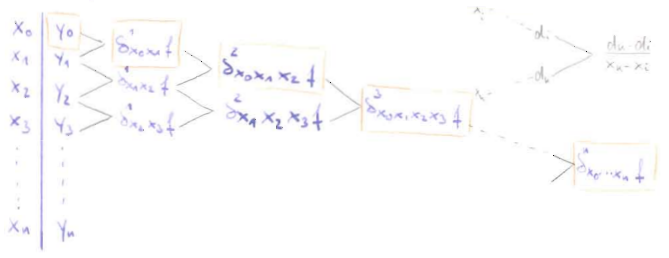
\includegraphics[scale=0.9]{2-interp-aitken.png}
\end{figure}

On admet le résultat que $P_n(X_i) = Y_i$ (démonstration par récurrence avec les formules de Newton).


Formule de Newton : identité algébrique pour toute fonction f
\begin{equation}
    % f(X) = 1 \cdot f(X_0) + (X - X_0) \delta_{X_0,X_1}^1 f + \cdots + (X - X_0) \cdot (X - X_1) \cdots (X - X_{n - 1}) \delta_{X_0,\cdots,X_n}^n f\\
    % + (X - X_0) \cdot (X - X_1) \cdots (X - X_n) \delta_{X,X_0,\cdots,X_n}^{n + 1} f
    f(X) = N_0(X) \cdot f(X_0) + N_1(X) \cdot \delta_{X_0,X_1}^1 f + \cdots + N_n(X) \cdot \delta_{X_0,\cdots,X_n}^n f + N_{n + 1}(X) \cdot \delta_{X,X_0,\cdots,X_n}^{n + 1} f
\end{equation}

Le dernier élément de $f(X)$ correspond au \og reste \fg, de degré (n + 1) dans la base de Newton.


\subsection* {Exemple}

\begin{figure}[h]
    \centering
    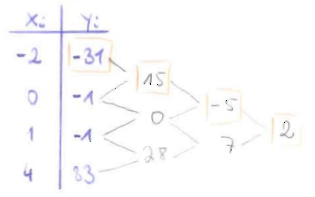
\includegraphics[scale=1.0]{2-interp-exemple.png}
\end{figure}

\begin{equation}
P_3(X) = -31 + 15 (X + 2) - 5 (X + 2) X + 2 (X + 2) X (X - 1)
\end{equation}

\subsection* {Résolution}

\begin{itemize}
\item Coût du tableau d'Aitken en $O(n^2)$ :

% $n + (n - 1) + \cdots + 2 + 1 = \sum_{i = 0}^n i = \frac{n (n + 1)}{2}$
$n + (n - 1) + \cdots + 2 + 1 = \frac{n (n + 1)}{2}$
\item $O(n)$ : évaluation du polynôme
\end{itemize}

\bigbreak
Cette méthode se prête à l'ajout de valeurs $(X_i, Y_i)$ à interpoler : il suffit de calculer autant de termes supplémentaires, alors qu'avec Vandermonde et Lagrange il faut tout recalculer.

\bigbreak
$\Rightarrow$ Donc la méthode de Newton est préférable à Vandermonde et Lagrange.

% Graphique Hermik


\section {Estimation de l'erreur}

Soit $f \in C^{n + 1}([a,b])$.

$\forall X \in [a,b], \xi \in [a,b]$, on a :

\begin{equation}
%\varepsilon(X) = 
f(X) - P_n(X) = \frac{f^{n + 1}(\xi)}{(n + 1)!} \cdot \prod_{i = 0}^n (X - X_i)
\end{equation}


\section {Problème de convergence}
\begin{equation}
\varepsilon_n = f(X) - P_n(X)
\end{equation}


$\varepsilon_n$ ne tend pas vers 0 quand n tend vers l'infini.

En effet, pour toute suite de $X_i$ on peut toujours construire une fonction continue pour laquelle l'interpolation polynomiale ne converge pas.


\section {Phénomène de Runge}

Il existe des fonctions qui montrent ce phénomène de convergence, exemple connu :
\begin{equation}
f(X) = \frac{1}{1 + X^2} \in [-5,5], f \in C^{\infty}
\end{equation}

\begin{figure}[h]
    \centering
    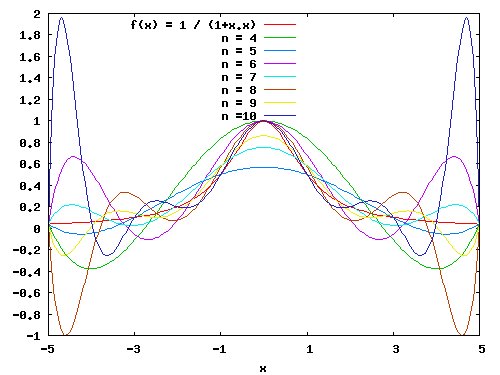
\includegraphics[scale=0.6]{2-interp-runge.png}
\end{figure}


\section* {Interpolation polynomiale}

\begin{itemize}
\item Adapté à un petit nombre n de valeurs à interpoler
\item Peu adapté aux données bruitées
\end{itemize}

On observe des problèmes d'oscillation sinon.

On peut diminuer ces problèmes avec un autre choix des abscisses $X_i$ (pas équidistantes) : les abscisses de Tchebychev.


\subsection* {Autre solution}

Interpolation par splines (par morceaux) de base avec différents degrés (ex : 3, 5).

% Graphique spline cubique



\chapter{Méthodes itératives pour des systèmes linéaires}

On sait aujourd'hui résoudre numériquement des systèmes linéaires de l'ordre du million d'inconnues (et d'équations). Pour des \textbf{systèmes creux}, c'est-à-dire lorsque la matrice du système possède beaucoup de coefficients nuls, on arrive à une centaine de millions d'inconnues.
Les \textbf{systèmes pleins} font appel à des \textbf{méthodes directes}, qui donnent la solution exacte (aux erreurs d'arrondi près) en un nombre fini d'itérations, et seront décrites dans un chapitre ultérieur.

Pour les \textbf{très grands systèmes creux\footnote{Exemple : discrétisation par différences finies de problèmes aux limites pour des équations aux dérivées partielles ...}}
on utilise des \textbf{méthodes itératives}, où on construit une suite de vecteurs qui convergent vers la solution.

L'intérêt est que \textbf{ces méthodes ne manipulent pas la matrice}, mais seulement une fonction qui définit une suite par récurrence.

\begin{fdef}
    Soit $A \in M_n(\R)$ inversible et $b \in \R^n$. On appelle méthode itérative de résolution du système linéaire $Ax=b$, ($x \in \R^n$) 
    une méthode qui construit une suite récurrente $(x_k)_{k\geq0}$
    telle que $$(x_k \underset{k\to +\infty}{\longrightarrow} x) \Rightarrow Ax=b$$
    Une méthode itérative est convergente si $x_k \underset{k\to +\infty}{\longrightarrow}x$ pour toute condition initiale $x_0 \in \R^n$
\end{fdef}

\underline{Tests d'arrêt typiques :}

% Pour les listes à puces, met un point noir en Énum
\renewcommand{\labelitemi}{\textbullet}
\begin{itemize}
    \item $\frac{\|Ax_k - b \|}{\|b\|} < \varepsilon$ (norme du ``résidu'' / norme de b).

        Noter que : 
        \begin{align*} \frac{\|x_k-x\|}{\|x\|} 
            = \frac{\|A^{-1}(Ax_k-b)\|}{\|x\|} 
            & \leq \|A^{-1}\| \frac{\|b\|}{\|x\|}\varepsilon 
            \\ & \leq \|A^{-1}\| \|A\| \varepsilon, 
            \; \mbox{peut-être grand !}\end{align*}

\end{itemize}


Nous allons décrire ici des méthodes itératives avec ``splitting'' de A.


\section{Description générale :}

On considère ici le système
\begin{equation}
    \label{eq:eqdiff}
    Ax = b
\end{equation} 
où $A \in M_n(\R)$, $x \in \R^n$ et $b \in \R^n$. On suppose que la matrice $A$ est inversible.


On considère une décomposition de A (``splitting'') $A=M-N$ avec $M$ inversible et on considère l'itération :

\begin{equation}
\left\lbrace
\begin{array}{ccc}
    Mx_{k+1} & = & Nx_k + b\\
    \\
    x_0 \in \R^n
    \label{eq:2}
\end{array}\right.
\end{equation}

Si $x_k \to x$ quand $k \to +\infty$ alors $Mx = Nx + b$, càd $x$ est solution de \reff{eq:eqdiff}.

Le choix du splitting est très important pour la performance de la méthode :
\begin{itemize}
    \item Bien sûr la méthode doit être convergente (voir plus loin)
    \item On doit choisir $M$ de telle sorte que le système \reff{eq:2} soit beaucoup plus facile à résoudre que \reff{eq:eqdiff} (il faut résoudre \reff{eq:2} à chaque étape de l'itération).

        \underline{Exemples :} $M$ diagonale ou triangulaire, diagonale ou triangulaire par blocs.
\end{itemize}

Étudions les conditions de convergence de \reff{eq:2}.

\begin{fdef}
    Étant donné $A \in M_n(\C)$, on note $S_p(A)$ l'ensemble des valeurs propres de $A$ (ou ``spectre de A''). On appelle rayon spectral de $A$ et on note $\rho(A)$ :
\[
    \rho (A) = \underset{\lambda \in S_p(A)}{\Max|\lambda|}
\]
\end{fdef}

\begin{ftheo}
    La méthode \reff{eq:2} converge si et seulement si $$\rho(M^{-1}N) < 1$$
\end{ftheo}

La preuve complète de ce résultat sera étudiée en TD. Ici nous allons simplement montrer que $\rho(M^{-1}N)<1 \Rightarrow $ convergence de \reff{eq:2}, en admettant pour cela deux résultats.

\vspace{1cm}

\begin{ftheo}[de l'application contractante (dans $\R^n$) ]
    Soit $E$ un sous-ensemble de $\R^n$ fermé (et non vide). On considère une norme $\| \, \|$ sur $\R^n$.

    Soit $F : E \rightarrow E$ une application contractante, càd pour laquelle il existe $\alpha \in [0,1[$ tel que :
\[
    \| F(x) - F(y) \| \leq \alpha \| x-y \| \mbox{,} \: \: \forall x,y \in E
\]

    Alors il existe un unique $x^* \in E$ tel que $F(x^*)=x^*$ (càd $F$ admet un unique point fixe dans E). De plus, pour tout $x_0 \in E$, la suite définie par :
\[
    x_{k+1} = F(x_k)
\]
converge vers $x^*$, avec
\begin{equation}
    \| x^* - x_k \| \leq \frac{\alpha^k}{1 - \alpha} \| x_1 - x_0 \|
    \label{eq:3}
\end{equation}

Le système \reff{eq:2} s'écrit :

\begin{equation}
\left\lbrace
\begin{array}{c}
    \boxed{x_{k+1} = M^{-1}N x_k + M^{-1} b}\\
    \\
    x_0 \in \R^n
    \label{eq:5}
\end{array}\right.
\end{equation}

\end{ftheo}

\begin{remark}
   Théorème encore appelé ``Théorème du point fixe de Banach''. Le théorème reste vrai lorsque $E$ est un espace métrique complet.
\end{remark}

\begin{ftheo}[cf TD pour la démonstration]
    Soit $A \in M_n(\C)$ et $\varepsilon > 0$. Il existe une norme $\| \, \|$ sur $\C^n$ telle que :
\[
    \underbrace{\|A\|}_
    \text{\parbox[]{2cm}{norme sur $M_n(\C)$ induite par la norme $\| \, \|$ de $C^n$}}
        :=  \underset{\|x\|=1}{\Sup} \|Ax\| \leq \rho(A) + \varepsilon
\]
  
\end{ftheo}

Si $\rho (M^{-1}N) < 1$, il existe donc une norme matricielle induite telle que $\| M ^{-1} N \| \leq \rho (M^{-1} N) + \varepsilon < 1$. Alors :
\[
    \| F(x) - F(y) \| = \| M^{-1} N (x-y) \| \leq \underbrace{\| M^{^-1}N \|}_{< 1} \| x-y \|
\]

Donc $F : \R^n \rightarrow \R^n$ est une contraction.

Donc $\forall x_0 \in R^n$, la suite définie par \reff{eq:5} converge vers une limite $x \in \R^n$ unique, solution de $x = M^{-1}Nx+M^{-1}b$, c'est-à-dire $Ax=b$.

% Je ne sais pas comment présenter ces points
\vspace{1cm}
\underline{Vitesse de convergence :} Plus $\rho(M^{-1}N)$ est petit, plus $\|M^{-1}N\|$ peut être choisie petite et plus la convergence est rapide.
En effet, d'après \reff{eq:3} :
\[
    \|x-x_k\| \leq \frac{\|M^{-1}N\|^k}{1-\|M^{-1}N\|}\|x_1-x_0\|
\]

\vspace{1cm}
\underline{Exemple de splitting : } (peu utilisé)
\[
    M = \frac{1}{\alpha}I, \qquad N = \frac{1}{\alpha}I - A \qquad \Longrightarrow \qquad x_{k+1} = (I - \alpha A)x_k + \alpha b
\]
(méthode de Richardson stationnaire, ou du gradient à pas fixe)

Elle converge si et seulement si $\forall \lambda \in Sp(A), |1-\alpha \lambda | < 1$, c'est-à-dire toutes les valeurs propres de A se trouvent dans le disque (ouvert) de centre $(\frac{1}{\alpha}, 0)$ et de rayon $\left| \frac{1}{\alpha} \right|$.

\section{Méthode de Jacobi}
On pose dans le schéma \reff{eq:2} :
\[
    M = D \mbox{ avec $D$ diagonale et } d_{ii}=a_{ii}, \qquad N=D-A
\]

On a donc :
\begin{equation}
D \cdot x_{k+1} = (D-A) \cdot x_k + b
\end{equation}
\begin{equation}
x_{k+1} = (I - D^{-1}A) \cdot x_k + D^{-1} b
\end{equation}

\begin{remark}
    Cela suppose $a_{ii} \ne 0 \; \forall i$ (si cette condition n'est pas vérifiée on peut permuter des lignes de $A$).
\end{remark}

En notant $x_k = (x^{(k)}_1,\dots,x^{(k)}_n)$ on obtient pour $i=1 \cdots n$ :
\begin{equation}
x^{(k+1)}_i = - \sum_{j \ne i}\frac{a_{ij}}{a_{ii}} \cdot x_j^{(k)} + \frac{b_i}{a_{ii}}
\end{equation}

\begin{ftheo}
    Si $A$ est à diagonale strictement dominante ($\rightarrow a_{ii}>0$ et $D$ inversible) alors la méthode de Jacobi converge.
\end{ftheo}

La démonstration sera vue en TD. On montre que le rayon spectral $\rho(J)$ de la matrice de Jacobi $J = D^{-1}N = D^{-1}(D-A) = I - D^{-1}A$ est $< 1$.

Nous avons rencontré ce type de matrices pour la discrétisation de problèmes aux limites dans le $1^{er}$ chapitre du cours.

\section{Méthode de Gauss-Seidel}

On suppose $a_{ii} \ne 0$, $\forall i = 1 \cdots n$.
\begin{itemize}
\item Méthode souvent plus rapidement convergente que celle de Jacobi
\item + économique en terme de stockage : un seul vecteur à stocker pour le calcul de l'itéré suivant
\item Converge pour les matrices symétriques définies positives (pas le cas pour Jacobi)
\end{itemize}

On pose $A = L + D + U$ avec :

\[
   L =
   \begin{pmatrix}
        0        & \cdots & 0      \\
        \vdots   & \ddots & \vdots \\
        a_{ij}(i>j)      & \cdots & 0
   \end{pmatrix}
   , D =
   \begin{pmatrix}
       a_{11} & \cdots                      & 0      \\ 
       \vdots & a_{ii}\hspace{-0.5cm}\ddots & \vdots \\ 
       0      & \cdots                      & a_{nn}
   \end{pmatrix}
   , U =
   \begin{pmatrix}
        0        & \cdots & a_{ij}(j>i)     \\
        \vdots   & \ddots & \vdots \\
        0        & \cdots & 0
   \end{pmatrix}
\]

Dans la méthode de Gauss-Seidel, on fixe :
\[
    M = L + D, \; N = -U
\]
\[
    \Rightarrow A = M - N
\]

La méthode s'écrit donc :
\[
    Dx_{k+1} = -Lx_{k+1}-Ux_k + b
\]
En notant $x_k = (x^{(k)}_1,\dots,x^{(k)}_n)$ on obtient pour $i = 1 \cdots n$ :
\[
    a_{ii}x^{(k+1)}_i = - \sum_{j<i}a_{ij}x_j^{(k+1)} - \sum_{(j>i)}a_{ij}x_j^{(k)} + b_i
\]

\begin{ftheo}
    Si $A$ est à diagonale strictement dominante alors la méthode de Gauss-Seidel converge.
\end{ftheo}

\begin{ftheo}
    Si $A$ est symétrique définie positive (SDP) alors la méthode de Gauss-Seidel converge.
\end{ftheo}

A est SDP $\Leftrightarrow$ $^txAx > 0, \forall x \ne 0$


\section{Méthode SOR}

Les méthodes de Jacobi et Gauss-Seidel ne sont guère utilisées. On leur préfère la méthode de relaxation.

La méthode SOR (``successive over-relaxation'', ou ``méthode de relaxation'', environ 1950) généralise Gauss-Seidel en introduisant un paramètre de relaxation $\omega \ne 0$,
que l'on ajuste afin d'accélérer la convergence de la méthode (avec un gain généralement très important si $\omega$ est bien choisi).

Pour $i=1,\dots,n$
\begin{equation}
\left\lbrace
\begin{array}{ccc}
    a_{ii}\tilde{x}_i^{(k+1)} & = & -\sum_{j<i} a_{ij}x_j^{(k+1)} - \sum_{j>i}a_{ij}x_j^{(k)} + b_i\\
    x_i^{(k+1)} & = & \omega \tilde{x_i}^{(k+1)} + (1-\omega)x_i^{(k)}
    \label{eq:4}
\end{array}\right.
\end{equation}
(Gauss-Seidel correspond à $\omega = 1$)

La méthode s'écrit (multiplier la seconde ligne par $a_{ii}$, et remplacer $a_{ii}\tilde{x_i}^{(k+1)}$ par son expression en fonction de $x_{k+1}$ et $x_k$)

\[
    Dx_{k+1}=(1-\omega)Dx_k - \omega L x_{k+1} - \omega U x_k + \omega b
\]

soit

\[
    (D + \omega L)x_{k+1} = [(1-\omega)D - \omega U]x_k + \omega b
\]

On a donc : 
\[
    M = \frac{1}{\omega}D + L, N = \frac{1-\omega}{\omega}D - U, M-N=D+L+U=A
\]

On note :
\[
    \mathcal{L}_{\omega} := (\frac{1}{\omega}D + L)^{-1}(\frac{1-\omega}{\omega}D - U)
\]
SOR converge si $\rho(\mathcal{L}_{\omega}<1$)

\begin{ftheo}[demo en TD]
    \begin{enumerate}
        \item
            Soit $A \in M_n(\R)$ inversible, avec $\forall i, a_{ii} \ne 0$
            Une condition nécessaire pour que SOR converge est que $\omega \in ]0,2[$.

        \item
            Si A est symétrique définie positive, alors $\forall \omega \in ]0,2[$, SOR converge 
    \end{enumerate}
\end{ftheo}

\begin{rappel}
    $A$ est symétrique définie positive si $A$ est symétrique, $^txAx = 0 \Rightarrow x = 0$, et $\forall x \in \R^n, {}^t\!xAx \geq 0$
\end{rappel}

\begin{coroll}
    Si $A$ est symétrique définie positive, alors la méthode de Gauss-Seidel converge.
    Nous avons rencontré ce type de matrices pour la discrétisation des problèmes aux limites dns le $1^{er}$ chapitre du cours (paragraphe 2), cas où la fonction $p$ est identiquement nulle.
\end{coroll}

\begin{remark}
    \begin{enumerate}
        \item Il y a des exemples où $A$ est symétrique définie positive et où la méthode de Jacobi n'est pas convergente.
        \item Si A est tridiagonale ($a_{ij}=0$ si $\abs{i-j}>1$) et $D$ inversible, on peut montrer que $\rho(\mathcal{L}_1)=\rho(J)^2$. Donc la méthode de Gauss-Seidel converge si et seulement si celle de Jacobi converge (et Gauss-Seidel converge plus vite).
        \item  Pour quelques types de matrices, on connaît la valeur de $\omega$ qui minimise $\rho (\mathcal{L}_{\omega})$.
            Pour $A$ tridiagonale (avec $D$ inversible), et si les valeurs propres de $J$ sont réelles, alors le paramètre de relaxation optimal dans SOR (c'est-à-dire la valeur de $\omega$ qui minimise $\rho (\mathcal{L}_{\omega})$) est > 1 (donc Gauss-Seidel ne donne pas la vitesse optimale de convergence).
        \item Pour optimiser empiriquement le choix de $\omega$ dans SOR, on peut évaluer le facteur de contractivité $\frac{\| x_{k+1} - x_k\|}{\| x_k - x_{k-1}\|}$ à partir du moment où $\|x_{k+1}-x_{k}\|$ décroît vers 0.
    \end{enumerate}
\end{remark}

\begin{figure}[h]
    \centering
    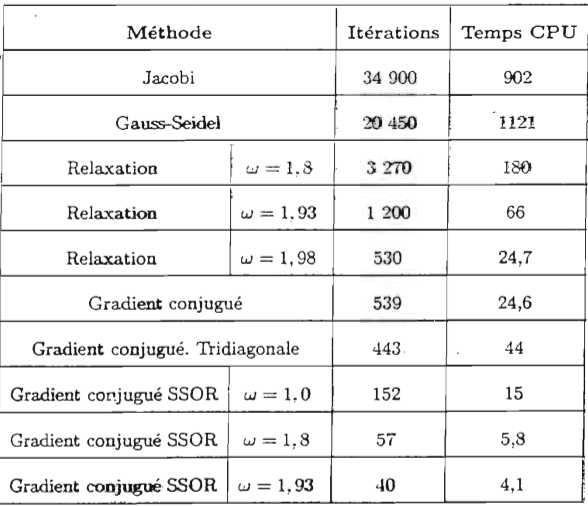
\includegraphics[scale=0.5]{tableau.png}
    \caption{Exemples pratiques}
    \label{fig:tableau}
\end{figure}


\chapter{Méthode de Gauss pour les systèmes linéaires et factorisation LU}
\chaptermark{Gauss pour systèmes linéaires et factorisation LU}

Soit $A \in M_n(\R)$ inversible et $b \in \R^n$. La méthode de Gauss permet de résoudre le système $Ax=b$, $x \in \R^n$ en se ramenant à la résolution d'un système triangulaire.
Nous allons commencer par rappeler cette méthode classique de résolution des systèmes linéaires. Il s'agit d'une \underline{méthode directe}, càd qui donne la solution exacte un nombre fini d'opérations arithmétiques élémentaires.
Nous verrons ensuite que l'élimination de Gauss fournit une factorisation $A = LU$ (ou $PA = LU$, $P$ étant une matrice de permutation, dépendant du choix des pivots)
avec $L$ triangulaire inférieure et $U$ triangulaire supérieure.
Résoudre $Ax=b \Leftrightarrow PAx = Pb \Leftrightarrow LUx = Pb$ revient donc à :

\begin{enumerate}
    \item Factoriser $PA$
    \item Résoudre $Lc = Pb$ (étape de \underline{descente}) $c_1 \to c_2 \to \dots \to c_n$
    \item Résoudre $Ux = c$ (étape de \underline{remontée}) : $x_n \to x_{n-1} \to \dots \to x_1$
\end{enumerate}

Si on doit résoudre de nombreuses fois avec la même matrice :
\[
    Ax^{(k)}=b^{(k)}
\]

Schémas ``implicites'' pour des EDP, schémas itératifs pour des systèmes linéaires ou non linéaires, \dots) alors l'étape 1) qui est la plus coûteuse est effectuée une seule fois.



\section{Rappel de l'élimination de Gauss :}

Soit $A \in M_n(\R)$ inversible et $b \in \R^n$. On cherche $x \in \R^n$ tel que $Ax=b$, soit :

\begin{equation}
    \left\lbrace
    \begin{array}{ccc}
        a_{11}X_1 + a_{12}X_2+ \dots+ a_{1n}X_n & = & b_1 \\
        \vdots \\
        a_{n1}X_1 + a_{n2}X_2 + \dots + a_{nn}X_n & = & b_n
    \end{array}\right.
\end{equation}


En notant $L_i = (a_{i1}, \cdots, a_{in})$ la i\up{ème} ligne de $A$, on a
\begin{equation}
    \left\lbrace
    \begin{array}{ccc}
        L_1 X = b_1 \\
        \vdots \\
        L_n X = b_n
    \end{array}\right.
    \tag{S}
    \label{eq:S}
\end{equation}


Si $a_{11} \neq 0$, on peut éliminer la variable $x_1$ dans les lignes 2 à $n$. On dit qu'on choisit $a_{11}$ comme \underline{pivot}.
$(S)$ équivaut à :
\[
    \left\lbrace
    \begin{array}{ccc}
        L_{1}X & = & b_1 \\
        (L_i - \frac{a_{i1}}{a_{11}}L_1) X & = & b_i - \frac{a_{i1}}{a_{11}}b_1 
    \end{array}\right.
    \hspace{2cm} i = 2..n
\]

Le nouveau système s'écrit $A^{(2)}X =b^{(2)}$ avec

\[
    A = 
    \begin{pmatrix}
        a_{11}^{(1)} & \cdots & a_{1n}^{(1)} \\
        0 \\
        \vdots \\
        0
    \end{pmatrix} 
    ,
    (a_{ij}^{(1)} = a_{ij})
\]

Ligne $i = L_i - l_{i1}L_1$ avec $l_{i1} = \frac{a_{i1}}{a_{11}}$

$b_i^{(2)} =  b_i - l_{i1}b_1$

Si $a_{11}$ on permute la 1ère ligne de \reff{eq:S} avec une autre ou $a_{i1} \neq 0$. Cela est toujours possible puisque $A$ est inversible.
On effectue la même procédure que précédemment expliqué.

Le système $A^{(2)} X = b^{(2)}$ contient un sous-système de dimension $n-1$ pour $x_2\dots x_n$
On répète la même procédure sur le sous-système pour éliminer $X_2$ des lignes 3 à $n$.

On continue ainsi et on déduit
\[
    A^{(3)}X = b^{(3)}, A^{(4)}X = b^{(4)}, \dots, A^{(n)}X=b^{(n)}
\]
Le dernier système obtenu est triangulaire. Notons $A^{(n)}=U$, $b^{(n)}=C$.

\begin{equation}
    \left\lbrace
    \begin{array}{ccccccc}
        u_{11}x_1 & + & \dots & + & u_{1n}x_n & = & c_1 \\
                  & u_{22}x_2 + & \dots & + & u_{2n}x_n & = & c_2 \\
        & & & \ddots \\
        & & & & u_{nn}x_n & = & c_n \\
    \end{array}\right.
    \tag{S'}
    \label{eq:S2}
\end{equation}

\reff{eq:S2} est facile à résoudre : \underline{``étape de remontée''}.
\[
    x_{nn} = \frac{c_n}{u_{nn}}, x_i = \frac{1}{u_{ii}}(c_i - \sum_{j=i+1}^{n}u_{ij}x_j )
\] pour $i = n-1, \dots, 1$

\begin{remark}
    On appelle \underline{``factorisation''} le calcul de $U$.
\end{remark}









\section{Factorisation LU}
Nous avons vu que l'élimination de Gauss peut conduire à permuter des lignes de A puisqu'on a besoin de ``pivots'' non nuls $a_{11}^{(1)}, a_{22}^{(2)}$ etc \dots Les cas où ces pivots sont voisins de 0 conduisent à des problèmes numériques (voir plus loin). Il est donc fréquent d'effectuer des permutations des lignes de A lors de l'élimination de Gauss.
Nous allons tout d'abord voir que ces permutations sont une traduction matricielle simple.

Notons ${p_1,p_2,\dots,p_n}$ une permutation des entiers ${1,2,\dots,n}$ et $(e_1,\dots,e_n)$ la base canonique de $\R^n$. On appelle \underline{matrice de permutation} une matrice de la forme :

\[
    P =
    \begin{pmatrix}[c|c|c|c]
        e_{p_1} & e_{p_2} & \dots & e_{p_n}\\
\end{pmatrix} 
\]

On a $p_{l_i} = e_{p_i}$ et :

\[
    P
    \begin{pmatrix}
        x_1 \\ x_2 \\ \vdots \\ x_n
    \end{pmatrix}
    =
    \begin{pmatrix}
        \vdots \\ \vdots \\ x_j \\ \vdots
    \end{pmatrix}
    \text{$\leftarrow$ ligne $p_j$}, \hspace{1cm}
    P
    \underbrace{\begin{pmatrix}
        L_1 \\
        L_2 \\
        \vdots \\
        L_n
    \end{pmatrix}
    }_\text{A}
    =
    \begin{pmatrix}
        \vdots \\
        \vdots \\
        L_j \\ 
        \vdots
    \end{pmatrix}
    \text{$\leftarrow$ ligne $p_j$}
\]

Soit $A \in M_n(\R)$. Notons $P$ la matrice correspondant aux permutations effectuées sur les lignes de $A$ dans l'algorithme du paragraphe \textbf{1}.
On a donc $PA = \tilde{A}$, où l'élimination de Gauss sur $\tilde{A}$ se fait sans permutation. Le passage de $A^{(j-1)}$ à $A^{(j)}$ s'écrit (même notations qu'auparavant) : 
\[
    \text{Ligne $i$} = L_i - L_j \times \left( \frac{a^{(j-1)}_{ij}}{a^{(j-1)}_{jj}} \right), \hspace{0.5cm} i = j+1, \dots , n
\]

Soit matriciellement :
\[
    A^{(j)} = T_j A^{(j-1)}, \hspace{0.5cm} T_j =
    \begin{pmatrix}[c|c]
        \begin{matrix}[ccc]
        & & \\
        & I_j & \\
        & & \\
        \end{matrix} 
        &
        \begin{matrix}
            \scalebox{1.5}{0}
        \end{matrix}
        \\ \hline
        \begin{matrix}[ccc|c]
            & & & -l_{j+1,j} \\
            & \scalebox{1.5}{0} & & \vdots \\
            & & & -l_{n,j}
        \end{matrix}
        &
        \begin{matrix}[ccc]
        & & \\
        & I_{n_j} & \\
        & & \\
        \end{matrix} 
    \end{pmatrix}
\]

\[
    l_{ij} = \frac{a^{(j-1)}_{ij}}{a^{(j-1)}_{jj}} , \hspace{0.5cm} I_k = \text{matrice identité de taille $k$}
\]

    En effet : 
\[
    \begin{blockarray}{cccc}
        \begin{block}{c(ccc)}
            & & 0 & \\
            \cline{2-4}
            & & 0 & \\
            \cline{2-4}
            \text{\scalebox{0.7}{ligne $i \rightarrow$}} & 0 \dots 0 & 1 & 0 \dots 0 \\
            \cline{2-4}
            & & 0 & \\
            \cline{2-4}
            & & 0 & \\
        \end{block}
        & & \text{\scalebox{0.7}{$\uparrow$ colonne $j$}} & & \\
    \end{blockarray}
    \times
    \begin{pmatrix}
        L_1 \\ \hline
        L_2 \\ \hline
        \vdots \\ \hline
        L_n
    \end{pmatrix}
    =
    \begin{pmatrix}
        0 \\ \hline
        0 \\ \hline
        L_j \\ \hline
        0 \\ \hline
        0
    \end{pmatrix} \text{$\leftarrow$ ligne $j$}
\]

On a donc :
\[
    U = A^{(n-1)} = T_{n-1} \times T_{n-2} \times \dots \times T_1 \times PA = TPA
\]
Avec $U$ triangulaire supérieure et $T$ triangulaire inférieure (produit de matrices triangulaires inférieures).

Donc on a $PA=LU$ avec $L=T^{-1}$ triangulaire inférieure (l'inverse d'une matrice triangulaire inférieure l'est aussi).

\begin{remark}
    Dans $\ref{eq:S2}$ on a $C=TPb$ et donc $LC=Pb$.
\end{remark}

% l_ij à afficher en plus grand ... 
Soit maintenant :\[
    \tilde{L} =
    \begin{pmatrix}
        1 & & \scalebox{1.2}{0} \\
        & \ddots & \\
        l_{ij} & & 1
    \end{pmatrix}
\]

On a : 
\[
    T_1 \tilde{L} =
    \begin{pmatrix}
        1      &        &        & 0 \\
        0      & 1      &        &   \\
        \vdots &        & \ddots &   \\
        0      & l_{ij} &        & 1
    \end{pmatrix}
    , \dots , T_{n-1} \times T_{n-2} \times T_1 \tilde{L} = I
\]

Donc $L = \tilde{L}$. Nous avons donc montré le résultat suivant :

\begin{ftheo}[Factorisation LU d'une matrice inversible]
    Soit $A \in M_n(\R)$ inversible. Il existe une matrice de permutation $P$
et deux matrices triangulaires L (triangulaire inférieure de diagonale unité) et $U$ (triangulaire supérieure inversible) telles que $PA = LU$.

    Cette décomposition est donnée explicitement par l'élimination de Gauss, avec 
    (les coefficients $l_{ij}$ sont ceux de l'élimination de Gauss sur $\tilde{A}$) :

    \[
        L = \begin{pmatrix}
            1 & & 0 \\
            & \ddots & \\
            l_{ij} & & 1 \\
        \end{pmatrix}
        , U =
        \begin{pmatrix}
            \ddots & & U_{ij} \\
            & \ddots & & \\
            0 & &
        \end{pmatrix}
    \]

    Cette factorisation est unique lorsque l'on fixe P.
    \label{th:factoLU}
\end{ftheo}

\begin{remark}
    L'unicité s'obtient simplement :
    $PA$ est inversible (puisque $P$ et $A$ le sont).

    Si $PA = L_1 U_1 = L_2 U_2$ alors $L_i$ et $U_i$ sont inversibles et donc
    $L^{-1}_2 L_1 = U_2 U^{-1}_1$. Le membre de droite est triangulaire supérieur, celui de gauche et triangulaire inférieur de diagonale unité.

    Donc $L^{-1}_2 L_1 = U_2 U^{-1}_1 = I$, i.e. $L1 = L2$ et $U_1 = U_2$.
\end{remark}

\vspace{0.7cm}
Les permutations effectuées lors de l'élimination de Gauss sont très importantes d'un point de vue numérique (voir plus loin).
Bien sûr, si l'on raisonne en arithmétique exacte (sans tenir compte des erreurs d'arrondi)
on voit dans l'algorithme de Gauss que les cas nécessiteant une permutation sont
exceptionnels (cela se produit lorsque $a_{11}$ ou $a^{(i)}_{i+1,i+1}=0$ pour certaines valeurs de $i$).

On a plus précisément le résultat suivant :

\begin{ftheo}
    Dans le théorème \ref{th:factoLU}, si les $n$ sous-matrices
    \[\Delta = \begin{pmatrix}
        a_{11} & \dots & a_{1i} \\
        \vdots & & \vdots \\
        a_{i1} & \dots & a_{ii}
    \end{pmatrix}
, (1 \leq i \leq n)\]
    sont inversibles, alors on peut fixer $P = I$.
\end{ftheo}

\begin{preuve}
    $a_{11} \ne 0$ donc la 1\up{ère} de l'élimination de Gauss ne nécessite pas de permutation.
    Supposons qu'on ait $j$ étapes sans permutation :
    \[
        A^{(j)} =
        \begin{pmatrix}[c|c]
            U^{(j)} & X \\ \hline
            0 & X
        \end{pmatrix}
        = T_j T_{j-1} \times \dots \times T_1 \times A =
        \begin{pmatrix}[c|c]
            \begin{matrix}
                1 & & 0 \\
                & \ddots & \\
                X & & 1
            \end{matrix}
            & \begin{matrix}[ccc]\\ & 0 & \\ \end{matrix}
            \\ \hline
            \begin{matrix}[ccc]\\ & X & \\ \end{matrix}
            & \begin{matrix}[ccc]\\ & I & \\ \end{matrix}
        \end{pmatrix}
        \begin{bigmatrix}{2.5}{c|c}
            \Delta_j & X \\
            \hline
            X & X
        \end{bigmatrix}
    \]
    avec $U^{(j)} \in M_j(\R)$ de la forme 
    $\begin{pmatrix} 
        a_{11} & & & X \\
        & a_{22}^{(1)} & & \\
        & & \ddots & \\
        0 & & & a_{jj}^{(j)}
    \end{pmatrix}$
    (les coefficients diagonaux sont les pivots).

    Alors on a aussi :
    \[
        %%%
        A^{(j)} =
        \begin{pmatrix}[c|c]
            \begin{matrix}[ccc]
                \\
                & U^{(j+1)} & \\
            \end{matrix}
            &
            \begin{matrix}[ccc]
                \\
                & X & \\
            \end{matrix}
            \\ \hline
            \begin{matrix}[cc|c]
               \\
               0 & & X \\
            \end{matrix}
            &
            \begin{matrix}[ccc]
                \\
                & X & \\
            \end{matrix}
        \end{pmatrix}
        %%%
        =
        %%%
        \begin{pmatrix}[c|c]
            \begin{matrix}
                1 & & 0 \\
                & \ddots & \\
                X & & 1
            \end{matrix}
            & \begin{matrix}[ccc]\\ & 0 & \\ \end{matrix}
            \\ \hline
            \begin{matrix}[ccc]\\ & X & \\ \end{matrix}
            & \begin{matrix}[ccc]\\ & I & \\ \end{matrix}
        \end{pmatrix}
        \begin{bigmatrix}{2.5}{c|c}
            \Delta_{j+1} & X \\
            \hline
            X & X
        \end{bigmatrix}
    \]

    avec $U^{(j+1)} = 
    \begin{pmatrix} 
        a_{11} & & & X \\
        & a_{22}^{(1)} & & \\
        & & \ddots & \\
        0 & & & a_{j+1,j+1}^{(j)}
    \end{pmatrix}$.
    Donc $U^{(j+1)} = 
            \begin{pmatrix}
                1 & & 0 \\
                & \ddots & \\
                X & & 1
            \end{pmatrix}
            \times \Delta_{j+1}$
            
            D'où : $a_{11} \times a_{22}^{(1)} \times \dots \times a^{(j)}_{(j+1),(j+1)} = \Det U^{(j+1)} = \Det \Delta_{j+1} \ne 0$ 
\end{preuve}

Donc $a^{(j)}_{j+1,j+1} \ne 0$ et on peut choisir ce coefficient comme pivot pour l'étape $j+1$.

Par récurrence, on peut donc choisir les coefficients $a_{11}, a_{i+1,i+1}^{(i)}$ comme pivots, puisque tous ces coefficients sont $\ne 0$. On obtient donc le résultat du théorème \ref{th:factoLU} avec $P=I$.


\begin{remark}
    Les coefficients $l_{ij}$ du théorème \ref{th:factoLU} sont ceux qui apparaissent dans l'élimination de Gauss faite sur $\tilde{A}$. Cependant, ils peuvent aussi se calculer directement à partir de l'élimination de Gauss faite sur A. Pour cela, quand on permute deux lignes de $A$, on réalise la même permutation sur les coefficients $l_{ij}$ calculés précédemment (cf TD pour un exemple).

    La remarque suivante détaille pourquoi ce procédé fonctionne.
\end{remark}

\begin{remark}[Permutation des coefficients $l_{ij}$ lors de l'élimination de Gauss]
    Soit $P$ la matrice de permutation telle que $P_{l_{i}} = e_{P_i}$.
    Alors :
    \[
        \begin{pmatrix}[c|c|c|c]
            c_1 & c_2 & \dots & c_n
        \end{pmatrix}
        .
        P
        =
        \begin{matrix}[cc]
        \begin{pmatrix}[cc|c|cc]
            & & c_{p_i} & & 
        \end{pmatrix}
        \end{matrix}
        \text{ $\leftarrow$ colonne $i$}
    \]
(prendre la transposée du membre de droite et appliquer le résultat donné précédemment)

Dans l'élimination de Gauss, lorsqu'on effectue sur $A^{(j-1)}$ une combinaison linéaire de lignes, puis une permutation des lignes $j+1$ et $k$, on multiplie $A^{(j-1)}$ par :
\begin{figure}[h]
    \centering
    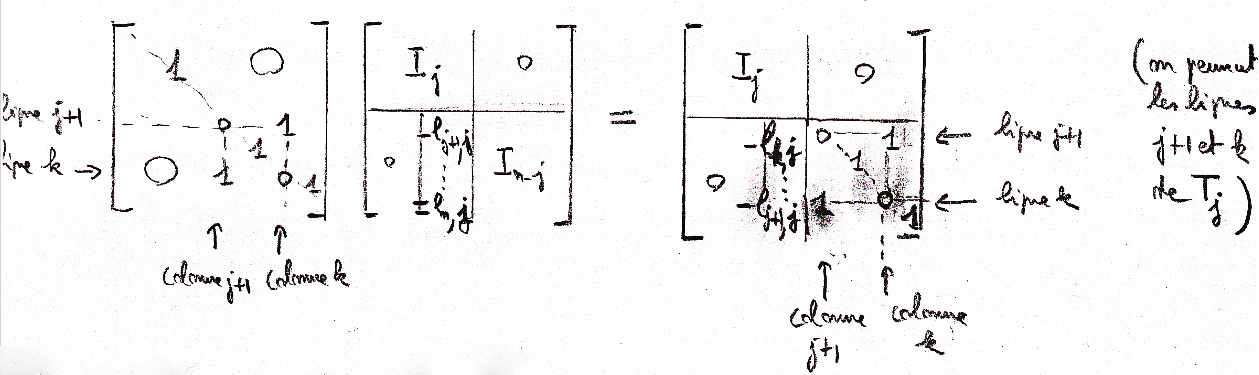
\includegraphics[scale=0.33]{matrices1.png}
\end{figure}

Cela revient au même de faire d'abord la permutation des lignes de $A^{(j-1)}$ puis la
combinaison linéaire où l'on permute les coefficients $l_{k,j}$ et $l_{j+1,j}$ (cf la
propriété de $P$ donnée plus loin : on permute les colonnes $j+1$ et $k$ de $T_j$).
\begin{figure}[h]
    \centering
    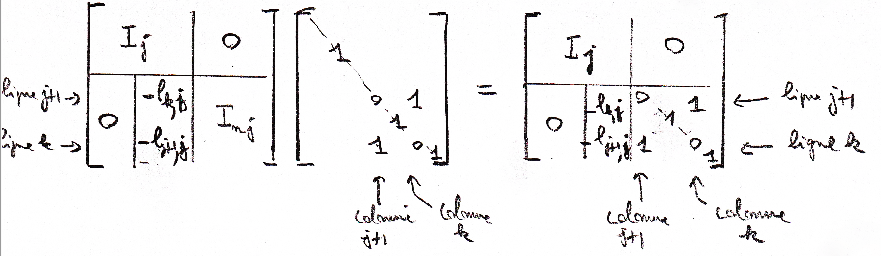
\includegraphics[scale=0.45]{matrices2.png}
\end{figure}

Donc les coefficients $l_{ij}$ du théorème 1 (coefficients de l'élimination de Gauss faite
sous permutation sur $PA$) s'obtiennent par permutation des coefficients $l_{ij}$ du
paragraphe 1) correspondant à l'élimination de Gauss sur la matrice $A$.
\end{remark}



\section{Techniques de choix du pivot}

Le choix d'un pivot non nul mais très petit peut conduire à des erreurs numériques importantes.
Par exemple, le système :
\begin{equation*}
    \left\lbrace
    \begin{array}{c}
        \varepsilon \; x_1 + x_2 = 1 \\
        x_1 + x_2 = 0 
    \end{array} \right.
\end{equation*}
a pour $\varepsilon \ne 1$ une solution unique $x_1 = -x_2 = \displaystyle\frac{1}{\varepsilon - 1}$

\begin{enumerate}[label=-]
    \item Si on résout (\ref{eq:S}) par la méthode de Gauss en utilisant $\varepsilon$ comme
        pivot, on obtient le système équivalent :
            \begin{align}
                \label{eqpivot1}
                \varepsilon \; x_1 = \; & 1 - x_2  \\
                x_2 (\frac{1}{\varepsilon} - 1) = \; & \frac{1}{\varepsilon} 
                \label{eqpivot2}
            \end{align}
\end{enumerate}

Par exemple , fixons $\varepsilon = 10^{-6}$. On simule un calcul
en virgule flottante avec 5 chiffres significatifs. Alors
$\frac{1}{\varepsilon} = 0,1.10^{7}$ (valeur exacte : $0,999999.10^6$)
d'où $x_2 = 1$ (valeur exacte : $x_2 = 10 \times \frac{100000}{999999} = 1,000001000001\dots$).

Mais alors $x_1 = 0$, ce qui est complètement faux (valeur exacte :
$x_1 = -x_2$).

Dans le membre de droite de (\ref{eqpivot1}), on effectue une 
soustraction qui est très mal conditionnée car $x_2 \approx 1$. Dans le calcul à
virgule flottante, on a $1 - x_2 = 0$, alors que la valeur exacte est 
$1 - x_2 \approx - 10^6$; on commet donc une erreur relative de $100 \%$,
alors que $x_2$ est connu avec une erreur relative de $10^{-6}$.

Si on choisit 1 comme pivot, on obtient :

\begin{equation*}
     \left \lbrace
     \begin{array}{ccc}
         x_1 + x_2  = & 0 \\[7pt]
         (1 - \varepsilon) x_2  = & 1
     \end{array}
     \right.
\end{equation*}

Alors $-\varepsilon + 1 = +0,1.10^1$ en virgule flottante (valeur exacte
$+0,999999$ d'où $x_2 = +1$ (précision $\sim 10^{-6}$) et $x_1 = -1$ (précision
$\sim 10^{-6}$).

Cela motive la :

\subsection*{Méthode de Gauss avec pivot partiel}
Même lorsque $a_{11} \ne 0$, on permute la 1\up{ère} ligne de (\ref{eq:S}) avec la
ligne où $|a_{i1}|$ est le plus grand. La même stratégie est répétée pour tous les
sous-systèmes apparaissant dans l'élimination de Gauss.

\begin{remark}
    Il existe aussi une méthode de Gauss avec pivot total, où on choisit comme
    pivot $a_{i_0,j_0}$ avec $|a_{i_0,j_0}| = \Max |a_{ij}|$.

    On permute alors la 1\up{ère} ligne de (\ref{eq:S}) avec la ligne $i_0$, et on
    permute les inconnues $x_1$ et $x_{j_0}$. On répète ce procédé pour tous
    les sous-systèmes qui apparaissent ensuite dans l'élimination de Gauss.

    La méthode avec pivot partiel est la plus employée. Elle marche bien en pratique.
    La méthode avec pivot total est plus coûteuse en temps de calcul; elle est donc
    assez peu employée.
\end{remark}


\section{Le coût de la méthode de Gauss}

\begin{eqnarray}
    \begin{split}
        Ax = b & \Leftrightarrow & PAX = Pb \\
        & \Leftrightarrow & LUX = Pb
    \end{split}
    \label{S1}
\end{eqnarray}

Résoudre \ref{S1} en 3 étapes :
\begin{enumerate}
    \item Factoriser $A$ ($PA = LU$)
    \item Résoudre $LC = Pb$ (méthode de remontée)
    \item Résoudre $UX = c$ (méthode de descente)
\end{enumerate}

\vspace{1cm}
\begin{remark}
    \begin{enumerate}
        \item L'étape 1. est la plus coûteuse
        \item Utiliser Fact-LU quand on a plusieurs systèmes linéaires. Avec la même matrice à résoudre : $AX^{(i)}=b^{(i)}, \; i = 1,2 \dots$
    \end{enumerate}
\end{remark}

\vspace{1cm}

* Factorisation $A=LU \; \; \; (P=I)$, à l'étape 1 de la factorisation : passage $A \to A^{(2)}$

\begin{enumerate}
    \item $(n-1)$ divisions (calcul de $l_{21}, \dots, l_{n1}$
    \item $2n(n-1)$ multitplications et additions (calcul $a_{ij}-l_{i1}a_{1j}, 2 \leq i \leq n, 1 \leq j \leq n$
    \item Passage $b$ à $b^{(2)}$, $2(n-1)$ multiplications et additions ($b_i - l_{i1}b_{1}, 2 \leq i \leq n$
\end{enumerate}

Il faut renouveler cette procédure pour les sous-systèmes de taille $n-1,n-2,\dots,2$

\underline{Au total}

\begin{equation*}
    \begin{rcases}
        \sim 2 \sum_{i=1}^n (n-i)^2 = 2.\frac{1}{3}n (n-\frac{1}{2})(n-1) \hspace{2cm}& +, *\\
        \sim 3 \sum_{i=1}^n (n-i) = 3.\frac{1}{2}n(n-1) \hspace{2cm} & +,*,\div
    \end{rcases}
    \text{$\Rightarrow \frac{2}{3}n^3+O(n^2)$}
\end{equation*}

* Réoslution d'un système triangulaire (étape de remontée)
(schéma pas pris)
\[
    X_n = \frac{b_n}{U_{nn}}
    x_i = \frac{1}{U_{2i}}(b_i - \sum_{k=i+1}^n a_{iK}X_K
\]

\begin{equation*}
    \text{$O(n^2)$}
    \begin{lcases}
        1 + 2 + 3 + \dots + n - 1 & = & \sum_{i=1}^{n-1}i = \frac{1}{2}(n-1)(n-2)\\
        1 + 2 + 3 + \dots + n - 1 & = & \sum_{i=1}^{n-1}i = \frac{1}{2}(n-1)(n-2)\\
        \text{n divisions}
    \end{lcases}
\end{equation*}

$\Rightarrow$ Donc la méthode de Gauss nécessite $\frac{2}{3}n^3+O(n^2)$ opérations.

\vspace{0.5cm}
\begin{remark}
    \begin{enumerate}
        \item Le pivot partiel a un coût en $O(n^2)$.
            \begin{itemize}
                \item [$\rightarrow$] Trouver le max parmi $n,n-1, \dots, 2, 1$ coeff.
            \end{itemize}

        \item Le pivot total a un coût en $O(n^3)$
            \begin{itemize}
                \item [$\rightarrow$] Trouver le max parmi $n^2, (n-1)^2, \dots , 2^2, 1^2$ coeff.
            \end{itemize}
    \end{enumerate}
\end{remark}






% definit le type de document et ses options
\documentclass[a4paper,11pt]{article}

% des paquetages utiles classiques, en ajouter d'autres selon vos besoins
\usepackage[utf8]{inputenc}
\usepackage[T1]{fontenc}
\usepackage{amsmath}
\usepackage{amssymb,calc}
% \usepackage{fullpage}
% \usepackage{stmaryrd}
% \usepackage{url}
% \usepackage{xspace}
\usepackage[francais]{babel}

% Pour les matrices annotées ... 
\usepackage{blkarray}

% Pour les figures
\usepackage{graphicx}

% Pour les listes à puces
\usepackage{enumerate}

\usepackage{indentfirst}

% Évite un conflit entre french babel et enumitem
\frenchbsetup{StandardLists=true}

\usepackage[standard,framed]{ntheorem}
\usepackage{framed}

% Pour les matrices par blocs je crois ?
\makeatletter
\renewcommand*\env@matrix[1][*\c@MaxMatrixCols c]{%
  \hskip -\arraycolsep
  \let\@ifnextchar\new@ifnextchar
  \array{#1}}
\makeatother

% Pour annoter les matrices :
\usepackage{kbordermatrix} 
\renewcommand{\kbldelim}{(} % change default array delimiters to parentheses
\renewcommand{\kbrdelim}{)}


% Pour des matrices agrandies :
\newenvironment{bigmatrix}[2]{%
  \renewcommand*{\arraystretch}{#1}% 
  \begin{pmatrix}[#2]
}{%
  \end{pmatrix}
}

% Pour des commentaires à droite d'équations
\newenvironment{rcases}
  {\left.\begin{aligned}}
  {\end{aligned}\right\rbrace}

\newenvironment{lcases}
  {\left\lbrace\begin{aligned}}
  {\end{aligned}\right.}


\newcommand{\reff}[1]{(\ref{#1})}


\setlength{\parindent}{30pt}
\setlength{\parskip}{1ex}
\setlength{\textwidth}{15cm}
\setlength{\textheight}{24cm}
\setlength{\oddsidemargin}{0.2cm}
\setlength{\evensidemargin}{-.7cm}
\setlength{\topmargin}{-.5in}

% des commandes pratiques pour ecrire des maths :
\newcommand{\dx}{\,dx}
\newcommand{\dt}{\,dt}
\newcommand{\ito}{,\dotsc,}
\newcommand{\R}{\mathbb{R}}
\newcommand{\N}{\mathbb{N}}
\newcommand{\C}{\mathbb{C}}
\newcommand{\Z}{\mathbb{Z}}
\newcommand{\Poly}[1]{\mathcal{P}_{#1}}
\newcommand{\abs}[1]{\left\lvert#1\right\rvert}
\newcommand{\norm}[1]{\left\lVert#1\right\rVert}
\newcommand{\pars}[1]{\left(#1\right)}
\newcommand{\bigpars}[1]{\bigl(#1\bigr)}
\newcommand{\set}[1]{\left\{#1\right\}}
\newcommand{\tpo}[1]{\,^t#1}


\DeclareMathOperator{\Sup}{Sup}
\DeclareMathOperator{\Max}{Max}
\DeclareMathOperator{\Det}{Det}
\DeclareMathOperator{\diag}{diag}
\DeclareMathOperator{\Min}{Min}

%
%\lstset{
%  literate=%
%  {À}{{\`A}}1 {Â}{{\^A}}1 {Ç}{{\c{C}}}1%
%  {à}{{\`a}}1 {â}{{\^a}}1 {ç}{{\c{c}}}1%
%  {É}{{\'E}}1 {È}{{\`E}}1 {Ê}{{\^E}}1 {Ë}{{\"E}}1% 
%  {é}{{\'e}}1 {è}{{\`e}}1 {ê}{{\^e}}1 {ë}{{\"e}}1%
%  {Ï}{{\"I}}1 {Î}{{\^I}}1 {Ô}{{\^O}}1%
%  {ï}{{\"i}}1 {î}{{\^i}}1 {ô}{{\^o}}1%
%  {Ù}{{\`U}}1 {Û}{{\^U}}1 {Ü}{{\"U}}1%
%  {ù}{{\`u}}1 {û}{{\^u}}1 {ü}{{\"u}}1%
%}

\newlength\dlf
\newcommand\alignedbox[2]{
  % #1 = before alignment
  % #2 = after alignment
    &
    \begingroup
    \settowidth\dlf{$\displaystyle #1$}
    \addtolength\dlf{\fboxsep+\fboxrule}
    \hspace{-\dlf}
    \boxed{#1 #2}
\endgroup
}

%%%%% PACKAGE AMSTHM :
% \newtheoremstyle{definition}
%   {20pt}   % ABOVESPACE
%   {20pt}   % BELOWSPACE
%   {}  % BODYFONT
%   {0pt}       % INDENT (empty value is the same as 0pt)
%   {\bfseries} % HEADFONT
%   {.}         % HEADPUNCT
%   {5pt plus 1pt minus 1pt} % HEADSPACE
%   {}          % CUSTOM-HEAD-SPEC

\newframedtheorem{ftheo}[theorem]{Theoreme}

\theoremstyle{plain} % default
\theorembodyfont{\normalfont}
\newframedtheorem{fdef}[definition]{Définition}

\renewtheorem{remark}{Remarque}

\newframedtheorem{coroll}{Corollaire}

\newtheorem{rappel}{Rappel}

\newtheorem{preuve}{Preuve}

\title{\huge \bfseries Méthode de Gauss pour les systèmes linéaires et factorisation LU}
\date{}


\begin{document}
\maketitle

La méthode de Cholesky (ou Choleski) permet de résoudre des systèmes linéaires
dont la matrice est symétrique définie positive. On rappelle que
$A \in M_n(\R)$ est symétrique définie positive si et seulement si :
\begin{enumerate}
    \item $^tA = A$
    \item $^tXAX \geq 0, \forall x \in \R$
    \item $^tXAX = 0 \Rightarrow X = 0$
\end{enumerate}
Pour une matrice $A \in M_n(\R)$ symétrique, les propriétés 2) et 3) reviennent à supposer que toutes les valeurs propres de $A$ sont $> 0$.

On a également :
\begin{enumerate}
    \item $A$ définie positive $\Rightarrow$ $A$ inversible
    \item $A$ symétrique $\Rightarrow$ $A$ diagonalisable. $\exists P / A = P^{-1}DP$
    \item $A$ symétrique et définie positive $\Rightarrow$ toutes les valeurs propres de $A$ sont positives et réelles.
\end{enumerate}

Nous allons voir que les matrices pevuent se factoriser sous la forme $A = T\tpo{T}$ où
$T$ est triangulaire inférieure.

Pour résoudre $Ax = b$ ($x,b \in \R^n)$, càd $T\tpo{T}x=b$ on résout alors successivement :
\begin{equation*}
\left\lbrace
    \begin{array}{ccc}
        Ty  = & b & \text{ étape de ``descente''}\\
        \\
        \tpo{T}x  = & y & \text{ étape de ``remontée''}
    \end{array}
\right.
\end{equation*}

Cette méthode est bien sûr intéressante lorsqu'on doit résoudre plusieurs systèmes linéaires
avec des seconds membres $b$ différents, mais la même matrice $A$ (la factorisation est faite
une seule fois, et les étapes de descente et remontée pour chaque second membre).


\begin{ftheo}
    Soit $A \in M_n(\R)$ symétrique définie positive. Il existe (au moins) une matrice réelle triangulaire inférieure $T$ telle que :
    \[
        A = T \,^tT
    \]
    De plus, si on impose que les éléments diagonaux de T soient tous positifs, alors la factorisation $A = T \,^tT$ est unique.
\end{ftheo}


\begin{preuve}
    Les $n$ sous-matrices 
$\Delta _i =
\begin{pmatrix}
    a_{11} & \dots & a_{1i} \\
    \vdots & & \vdots \\
    a_{i1} & \dots & a_{ii}
\end{pmatrix}$
sont inversibles car elles sont symétriques définies positives. En effet, si 
$x =
\begin{pmatrix}
    x_1 \\
    \vdots \\
    x_i
\end{pmatrix}
$
et
$X =
\begin{pmatrix}
    x_1 \\
    \vdots \\
    x_i \\
    0 \\
    \vdots \\
    0
\end{pmatrix}
$
on a $\tpo{x} \Delta_i x = \tpo{X}AX$

Donc, d'après le théorème 2 du chapitre précédent, on a $A = LU$ avec $L$ triangulaire
inférieure de diagonale unité, et $U$ triangulaire supérieure inversible $(\rightarrow u_{ii} \ne 0 \forall i)$.
Notons $D = \diag{u_{ii}}$

On a : $A = \tpo{A} = \tpo{U} \tpo{L} = \underbrace{\tpo{U} D^{-1}}_\text{triang. inf de diagonale unité \hspace{0.2cm}}
\times
\underbrace{D \tpo{L}}_\text{triangulaire supérieure}$

Par unicité de la décomposition $LU$ il vient $D\tpo{L} = U$ et donc $A = L D \tpo{L}$. De plus, si $\tpo{L} V_i = e_i$

\[
    0 < \tpo{V_i} \, A \, V_i = \tpo{V_i} \, L \; D \; \tpo{L} \, V_i = \tpo{e_i} \, D \, e_i = u_{ii}
\]

Notons maintenant $\sqrt{D} = \diag{\sqrt{u_{ii}}}$. Alors $A = L \, \sqrt{D} \, \tpo{\sqrt{D}} \, \tpo{L}$,
c'est-à-dire $A = T \tpo{T}$ avec $T = L \sqrt{D}$.

L'unicité de la factorisation $A = T \tpo{T}$ vient de l'algorithme de calcul de $T$ décrit plus loin.
\end{preuve}


\subsection*{Calcul de T :}

T peut être calculé à partir d'une factorisation LU, mais on expose ici une méthode moins coûteuse en temps de calcul.

Puisque $A = T \tpo{T}$ avec $T$ triangulaire inférieure :

\[
    a_{ij} = \sum_{1 \leq k \leq \Min(i,j)} t_{ik} t_{jk}
\]

\begin{enumerate}[$-$]
    \item Calculons la 1\up{ère} colonne de $T$ à partir de celle de $A$ :
        \[
            a_{11} = t_{11}^2 \implies t_{11} = \sqrt{a_{11}} \hspace{1cm} 
            \text{($a_{11} > 0$ car $A$ symétrique définie positive)}
        \]
        Pour $i \geq 2$ :
        \[
            a_{i1} = t_{i1} t_{11} \implies t_{i1} = \frac{a_{i1}}{t_{11}}
        \]
    \item Supposons connues les colonnes $1$ à $p$ de $T$, et calculons la colonne $p+1$ :
        \begin{align*}
            & a_{p+1,p+1} = t_{p+1,p+1}^2 + \sum_{1 \leq k \leq p}(t_{p+1,k})^2 \to
            \text{calculés précédemment (colonnes 1 à $p$)} \\
            \implies & t_{p+1,p+1}^2 = a_{p+1,p+1} - \sum_{1 \leq k \leq p}(t_{p+1,k})^2 > 0 \hspace{0.5cm} \text{\underline{puisque $T$ existe}} \\
            \implies & t_{p+1,p+1} = \left(a_{p+1,p+1} - \sum_{1 \leq k \leq p}(t_{p+1,k})^2)\right)^{\frac{1}{2}}
        \end{align*}

        Pour $i \geq p+2$ :
        \begin{equation*}
            \begin{split}
                & a_{i,p+1} = t_{i,p+1} t_{p+1,p+1} + \sum_{1 \leq k \leq p}(t_{ik} t_{p+1,k})
            \hspace{1cm} \to \text{(calculés précédemment)} \\
                \implies & t_{i,p+1} = (a_{i,p+1} - \sum_{1 \leq k \leq p} t_{ik}t_{p+1,r} \frac{1}{t_{p+1,p+1}})
            \end{split}
        \end{equation*}

\end{enumerate}

\subsection*{Coût du calcul de T :}
On assimile l'extraction de racine carrée à une opération arithmétique élémentaire (ce qui est
une approximation, car cette opération est plus compliquée que les opérations élémentaires
$\times, +, -$ \dots).

Calcul de la 1\up{ère} colonne de $T$ : $n$ opérations.

Calcul de la $(p+1)$\up{ème} de $T$ :

\begin{enumerate}[$-$]
    \item Calcul de $t_{p+1,p+1}$ :
        \[
            \left.
            \parbox{4cm}{
                \begin{enumerate}[$*$]
                    \item $p$ multiplications
                    \item $p$ soustractions
                    \item $1$ racine
                \end{enumerate}
            }\right\rbrace \text{$2p+1$ opérations}
        \]

    \item Calcul de $t_{i,p+1} (p+2 \leq i \leq n)$ :
        \[
            \left.
            \parbox{4cm}{
                \begin{enumerate}[$*$]
                    \item $p$ multiplications
                    \item $p$ soustractions
                    \item $1$ divison
                \end{enumerate}
            }\right\rbrace \text{$2p+1$ opérations}
        \]
\end{enumerate}

$\to (n-p) \times (2p+1)$ opérations pour le calcul de la colonne $p+1$.

\begin{align*}
    \text{Coût total} & = \sum_{p=0}^{n-1} (n-p)(2p+1) \\
    & = (2n-1) \Bigg( \sum_{p=1}^{n-1}p \Bigg) + n^2 - 2 \sum_{p=1}^{n-1} p^2 \\
    & \sim_{n \to + \infty} n^3 - \frac{2}{3} n^3
\end{align*} 

Donc nombre d'opérations élémentaires $\sim_{n \to +\infty} \frac{1}{3}n^3$.
($\sim \frac{1}{6}n^3$ multiplications et $\frac{1}{6}n^3$ soustractions)


\subsection*{Coût de la résolution de $Ax = b$}

Le coût des étapes des descente et de remontée est $\mathcal{O}(n^2)$.

L'étape la plus coûteuse est donc la factorisation $A = T \tpo{T}$, et le coût total est $\sim \frac{1}{3}n^3$. C'est donc mieux que Gauss (coût $\sim \frac{2}{3}n^3)$.

\end{document}





% definit le type de document et ses options
\documentclass[a4paper,11pt]{article}

% des paquetages utiles classiques, en ajouter d'autres selon vos besoins
\usepackage[utf8]{inputenc}
\usepackage[T1]{fontenc}
\usepackage{amsmath}
\usepackage{amssymb,calc}
% \usepackage{fullpage}
% \usepackage{stmaryrd}
% \usepackage{url}
% \usepackage{xspace}
\usepackage[francais]{babel}

% Pour les matrices annotées ... 
\usepackage{blkarray}

% Pour les figures
\usepackage{graphicx}

% Pour les listes à puces
% \usepackage{enumitem}

\usepackage{enumerate}

\usepackage{indentfirst}

% Évite un conflit entre french babel et enumitem
\frenchbsetup{StandardLists=true}

\usepackage[standard,framed]{ntheorem}
\usepackage{framed}

% Pour les matrices par blocs je crois ?
\makeatletter
\renewcommand*\env@matrix[1][*\c@MaxMatrixCols c]{%
  \hskip -\arraycolsep
  \let\@ifnextchar\new@ifnextchar
  \array{#1}}
\makeatother

% Pour annoter les matrices :
\usepackage{kbordermatrix} 
\renewcommand{\kbldelim}{(} % change default array delimiters to parentheses
\renewcommand{\kbrdelim}{)}


% Pour des matrices agrandies :
\newenvironment{bigmatrix}[2]{%
  \renewcommand*{\arraystretch}{#1}% 
  \begin{pmatrix}[#2]
}{%
  \end{pmatrix}
}

% Pour des commentaires à droite d'équations
\newenvironment{rcases}
  {\left.\begin{aligned}}
  {\end{aligned}\right\rbrace}

\newenvironment{lcases}
  {\left\lbrace\begin{aligned}}
  {\end{aligned}\right.}


\newcommand{\reff}[1]{(\ref{#1})}


\setlength{\parindent}{30pt}
\setlength{\parskip}{1ex}
\setlength{\textwidth}{15cm}
\setlength{\textheight}{24cm}
\setlength{\oddsidemargin}{0.2cm}
\setlength{\evensidemargin}{-.7cm}
\setlength{\topmargin}{-.5in}

% des commandes pratiques pour ecrire des maths :
\newcommand{\dx}{\,dx}
\newcommand{\dt}{\,dt}
\newcommand{\ito}{,\dotsc,}
\newcommand{\R}{\mathbb{R}}
\newcommand{\N}{\mathbb{N}}
\newcommand{\C}{\mathbb{C}}
\newcommand{\Z}{\mathbb{Z}}
\newcommand{\gO}{\mathcal{O}}
\newcommand{\Poly}[1]{\mathcal{P}_{#1}}
\newcommand{\abs}[1]{\left\lvert#1\right\rvert}
\newcommand{\norm}[1]{\left\lVert#1\right\rVert}
\newcommand{\pars}[1]{\left(#1\right)}
\newcommand{\bigpars}[1]{\bigl(#1\bigr)}
\newcommand{\set}[1]{\left\{#1\right\}}
\newcommand{\tpo}[1]{\,^t#1}


\DeclareMathOperator{\Sup}{Sup}
\DeclareMathOperator{\Max}{Max}
\DeclareMathOperator{\Det}{Det}
\DeclareMathOperator{\diag}{diag}
\DeclareMathOperator{\Min}{Min}

%
%\lstset{
%  literate=%
%  {À}{{\`A}}1 {Â}{{\^A}}1 {Ç}{{\c{C}}}1%
%  {à}{{\`a}}1 {â}{{\^a}}1 {ç}{{\c{c}}}1%
%  {É}{{\'E}}1 {È}{{\`E}}1 {Ê}{{\^E}}1 {Ë}{{\"E}}1% 
%  {é}{{\'e}}1 {è}{{\`e}}1 {ê}{{\^e}}1 {ë}{{\"e}}1%
%  {Ï}{{\"I}}1 {Î}{{\^I}}1 {Ô}{{\^O}}1%
%  {ï}{{\"i}}1 {î}{{\^i}}1 {ô}{{\^o}}1%
%  {Ù}{{\`U}}1 {Û}{{\^U}}1 {Ü}{{\"U}}1%
%  {ù}{{\`u}}1 {û}{{\^u}}1 {ü}{{\"u}}1%
%}

\newlength\dlf
\newcommand\alignedbox[2]{
  % #1 = before alignment
  % #2 = after alignment
    &
    \begingroup
    \settowidth\dlf{$\displaystyle #1$}
    \addtolength\dlf{\fboxsep+\fboxrule}
    \hspace{-\dlf}
    \boxed{#1 #2}
\endgroup
}

%%%%% PACKAGE AMSTHM :
% \newtheoremstyle{definition}
%   {20pt}   % ABOVESPACE
%   {20pt}   % BELOWSPACE
%   {}  % BODYFONT
%   {0pt}       % INDENT (empty value is the same as 0pt)
%   {\bfseries} % HEADFONT
%   {.}         % HEADPUNCT
%   {5pt plus 1pt minus 1pt} % HEADSPACE
%   {}          % CUSTOM-HEAD-SPEC

\newframedtheorem{ftheo}[theorem]{Theoreme}

\theoremstyle{plain} % default
\theorembodyfont{\normalfont}
\newframedtheorem{fdef}[definition]{Définition}

\renewtheorem{remark}{Remarque}

\newframedtheorem{coroll}{Corollaire}

\newtheorem{rappel}{Rappel}

\newtheorem{preuve}{Preuve}

\title{\huge \bfseries Résolution numérique d'équations non linéaires}
\date{}


\begin{document}
\maketitle

De nombreux problèmes issus notamment de la physique conduisent à la résolution d'équations non linéaires,
\[
    f(x)=0, \; f \in \mathcal{C}^1(\R^n,\R^n)
\]

\section{Méthode des approximations successives}

À partir d'une équation $f(x) = 0$ ($f : \R^n \longrightarrow R^n$ de classe $\mathcal{C}^1$),
on peut se ramener à un problème de point fixe :
\begin{equation}
    x = \Phi(x)
    \label{eq:ptfixe}
\end{equation}
avec $\Phi : \R^n \longrightarrow \R^n$ de classe $\mathcal{C}^1$. On peut poser par exemple :
\begin{equation*}
    \Phi(x) = x - B f(x)
\end{equation*}
avec $B \in M_n(\R)$ inversible.

Pour résoudre (\ref{eq:ptfixe}), on se donne une condition initiale $x_0 \in \R^n$ (la plus proche possible d'une solution de (\ref{eq:ptfixe})) et on considère la méthode itérative :
\begin{equation}
    x_{k+1} = \Phi(x_k)
    \label{eq:methodeiterative}
\end{equation}

Nous allons étudier la convergence de ce type de méthodes itératives.

\begin{fdef}
    Soit $a$ un point fixe de $\Phi$ ($\Phi(a) = a$).
    \begin{enumerate}[i)]
        \item $a$ est stable au sens de Lyapunov si
            \[
                \forall \varepsilon > 0, \exists \eta \; / \; \norm{x_0 - a} < \eta \implies \norm{x_k - a} < \varepsilon \hspace{1cm} \forall k \geq 0
            \]

        \item $a$ est instable s'il n'est pas stable au sens de Lyapunov.

        \item $a$ est asymptotiquement stable s'il est stable au sens de Lyapunov et
            \[
                \exists r \; / \; \norm{x_0 - a} < r \implies x_k \xrightarrow{k \to +\infty} a
            \]
    \end{enumerate}
\end{fdef}

Lorsque $a$ est asymptotiquement stable, la méthode (\ref{eq:methodeiterative}) permet de calculer numériquement $a$ à partir d'une condition initiale $x_0$ ``suffisamment proche'' de $a$.

\begin{ftheo}
    Soit $\Omega$ un ouvert de $\R^n$ et $\Phi : \Omega \longrightarrow \R^n$ de classe $\mathcal{C}^1$.
    Soit $a \in \Omega$ un point fixe de $\Phi$, i.e. $\Phi(a) = a$. Alors :
    \begin{enumerate}[a)]
        \item Si $\rho \Big(D\Phi(a) \Big) < 1$ alors $a$ est asymptotiquement stable.
        \item Si $\rho \Big(D\Phi(a) \Big) > 1$ alors $a$ est instable.
    \end{enumerate}
\end{ftheo}

\begin{rappel*}
    $D\Phi(a) \in M_n(\R)$ est définie par :
    \[
        \left.
        \parbox{4cm}{
            \[
                D \Phi (a) = \left( \frac{\partial \Phi_i}{\partial x_j}(a) \right)_{1 \leq i,j \leq n}
            \]
        } \hspace{1cm} \right \rbrace
        \begin{tabular}{@{}c@{}}
            différentielle de $\Phi$ au point $a$, \\ matrice Jacobienne de $\Phi$ au point $a$ 
        \end{tabular}
     \]
\end{rappel*}

\begin{preuve}[du a)]
    Notons $x_k = a + e_k$.
    \begin{equation*}
        \left\lbrace
        \begin{array}{ccc}
            x_{k+1} = \Phi (x_k) & \implies & e_{k+1} = \Phi(a+e_k) - \Phi(a) \\
            a = \Phi(a)
        \end{array}
        \right.
    \end{equation*}

    On utilise un développement de Taylor à l'ordre 1 :
    \[
        \Phi(a+e_k) = \Phi(a) + D\Phi(a) e_k + \norm{e_k}\varepsilon(e_k)
    \]
    avec $\norm{\varepsilon(e_k)} \to 0$ quand $e_k \to 0$.


    \vspace{0.5cm}
    Donc $e_{k+1} = D\Phi(a) e_k + o(\norm{e_k})$.

    Si $\rho \big(D\Phi(a) \big) < 1$, il exsite une norme matricielle induite pour
laquelle $\norm{D\Phi(a)}<1$.

    Donc $\exists \eta > 0$ et $\alpha < 1$ tels que si $\norm{e_k} < \eta$ :
    \[
        \norm{e_{k+1}} \leq \alpha \norm{e_k}
    \]

    Donc si $\norm{e_0} < \eta$, $\norm{e_k} \leq \alpha^k \norm{e_0} \xrightarrow{k \to +\infty}0$
\end{preuve}

\begin{remark}
    \begin{enumerate}[-]
        \item Ce résultat donne la convergence \underline{locale} de la méthode :
              convergence de  $(x_k)$ vers un point fixe $a$ de $\Phi$ si
              $\rho \big(D\Phi(a) \big)<1$ et $\norm{x_0-a}$ assez petit.
        \item La solution de (\ref{eq:ptfixe}) n'est pas forcément unique.
        \item a) $\implies \norm{x_{k+1}-a} \leq \alpha \norm{x_k-a}$ avec
              $\alpha < 1$, et plus $\rho \big( D\Phi(a) \big)$ est petit, plus
              $\alpha$ est petit. On dit que la convergence est (au moins)
              \underline{linéaire}.
        \item Sous l'effet des termes non linéaires, dans certains cas la méthode
            numérique (\ref{eq:methodeiterative}) peut être localement convergente
            avec $\rho \big( D\Phi(a) \big) = 1$. \underline{Exemple :} $x_{k+1} = x_k - x_k^3$, point fixe 0 asymptotiquement stable.
    \end{enumerate}
\end{remark}

\subsection*{Critères d'arrêt :}
\begin{enumerate}[a)]
    \item
        On se donne une tolérance absolue $tol$ (on pourrait aussi travailler en relatif)
        \[
              \norm{x_k - x_{k-1}} < tol
        \]
        Cela indique également que $\norm{\Phi(x_{k-1} - x_{k-1})} < tol$,
        c'est-à-dire que $x_{k-1}$ est ``presque'' solution de $\Phi(x) = x$.
        
    \item Lorsque $\Phi$ est une contraction sur un sous-ensemble fermé $E$ de
          de $\R^n$, on sait que $\Phi$ admet un unique point fixe $a$ dans $E$.
          Si $\alpha \in ]0,1[$ désigne le facteur de contraction de $\Phi$ on
          montre que si $x_{k-1} \in E$ alors $\norm{x_k-a} \leq \frac{\alpha}{1-\alpha} \norm{x_k - x_{k-1}}$.
          
          Fixer le critère d'arrêt $\norm{x_k - x_{k-1}} < tol \times \big(\frac{1}{\alpha} - 1 \big)$ et $x_{k-1} \in E$ garantit que $\norm{x_k - a} < tol$.


    \item Un critère intéressant peut être obtenu lorsque :
        \[
        \frac{\norm{x_k - x_{k-1}}}{\norm{x_{k-1}-x_{k-2}}} \xrightarrow{k\to+\infty} \lambda \in ]0,1[ 
        \]

        Cette propriété est vérifiée avec $\lambda = \rho \big(D\Phi(a) \big)$ et pour
        presque toute condition initiale $x_0 \approx 0$ si $\lambda$ \underline{ou} $-\lambda$
        est une valeur propre réelle simple de $D\Phi(a)$, avec toutes les autres
        valeurs propres de module $< \lambda$.

        (alors $x_k = a + V.(\pm \lambda)^k + o(\lambda^k$), $V$ vecteur propre
        associé à $\pm \lambda$)

        Alors pour $k$ assez grand et $p \geq k$

        \begin{align*}
            & \norm{x_k - x_p} \leq \norm{x_k - x_{k+1}} + \norm{x_{k+1} - x_{k+2}}
            + \dots + \norm{x_{p-1}-x_p} \\ 
            \\
            \implies & \norm{x_k - a} \leq \sum_{j \geq k} \norm{x_j - x_{j+1}} \hspace{1cm} \text{(on fait tendre $p$ vers $+\infty$)}
        \end{align*}
        
        On fait maintenant l'approximation :
        \begin{align*}
            \sum_{j \geq k} \norm{x_j - x_{j+1}} & \simeq \norm{x_k - x_{k+1}} \times \sum_{j \geq 0} \lambda ^j \simeq \frac{\lambda}{1 - \lambda} \norm{x_k - x_{k-1}} \\
            & \simeq \frac{\norm{x_k - x_{k-1}}}{\norm{x_{k-1} - x_{k-2}}} \times \frac{1}{1-\frac{\norm{x_k - x_{k-1}}}{\norm{x_{k-1}-x_{k-2}}}} \norm{x_k - x_{k-1}} \\
            & = \frac{\norm{x_k - x_{k-1}}^2}{\norm{x_{k-1} - x_{k-2}} - \norm{x_k - x_{k-1}}}
        \end{align*}

        On en déduit le critère d'arrêt :
        \begin{equation*}
            \left\lbrace
            \begin{array}{c}
                \displaystyle\frac{\norm{x_k - x_{k-1}}^2}{\norm{x_{k-1} - x_{k-2}} - \norm{x_k - x_{k-1}}} < tol \\
                \\
                \norm{x_k - x_{k-1}} < \norm{x_{k-1} - x_{k-2}}
            \end{array}
            \right.
            \tag{c}
        \end{equation*}
\end{enumerate}


        Le théorème de convergence de la méthode des approximations successives suppose que $\rho \big( D\Phi(a) \big) < 1$. 
        Un choix tel que $\Phi(x) = x - B f(x)$ ($B \in M_n(\R)$ inversible) ne garantit pas
        que cette hypothèse soit respectée, et que le rayon spectral soit petit 
        (condition pour que la convergence soit rapide).

        Nous allons définir un choix astucieux de fonction $\Phi$ à partir de $f$, pour
        lequel $D\Phi(a) = 0$. Il s'agit de la méthode de Newton.

\section{Méthode de Newton}

    Soit $f : \R^n \longrightarrow \R^n$ de classe $\mathcal{C}^2$. On veut calculer
    numériquement une solution de l'équation :
    \begin{equation}
        f(x) = 0
    \end{equation}

    Le principe de la méthode de Newton est le suivant. Si $x_0 \in \R^n$ est une approximation de la solution $x$ recherchée,
    on linéarise $f$ autour de $x_0$ :
    \[
        f(x) \simeq f(x_0) + Df(x_0)(x-x_0)
    \]

    On calcule alors la solution $x_1$ de :
    \[
        f(x_0) + Df(x_0)(x_1 - x_0) = 0 
    \]

    Si $Df(x_0)$ est inversible, on obtient :
    \[
        x_1 = x_0 - Df(x_0)^{-1}f(x_0)
    \]

    Puis on prend $x_1$ comme nouvelle approximation de la solution et on recommence
    l'opération. Cela définit la méthode itérative :
    \begin{equation}
        x_{k+1} = x_k - Df(x_k)^{-1}f(x_k) \underset{\text{déf}}{=} \Phi(x_k)
        \label{eq:newton}
    \end{equation}

    \begin{remark}
        Numériquement on ne calcule pas $Df(x_k)^{-1}$ mais on résout à chaque étape le
        système linéaire donnant $x_{k+1}$ :
        \[
            Df(x_k)(x_{k+1} - x_k) = -f(x_k)
        \]
    \end{remark}

    \subsection*{Interprétation géométrique en dimension 1 :}

    \begin{figure}[h]
        \centering
        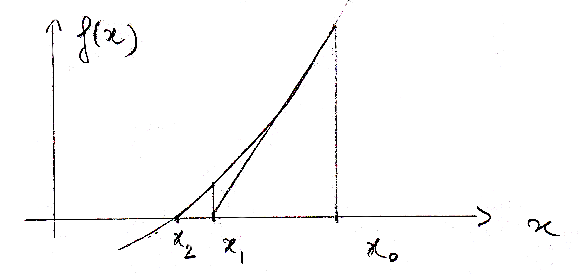
\includegraphics[scale=0.5]{newton-dim1.png}
    \end{figure}

    Nous sommes dans le cadre de la méthode des approximations successives :
    on cherche une solution de $\Phi(x) = x$ avec $\Phi(x) = x - Df(x)^{-1}f(x)$.
    La méthode itérative (\ref{eq:newton}) s'écrit $x_{k+1} = \Phi(x_k)$.


    \begin{ftheo}
        Soit $f : \R^n \longrightarrow \R^n$ de classe $\mathcal{C}^2$ au voisinage de $a \in \R^n$, avec $f(a) = 0$.
        On suppose que $Df(a)$ est inversible. Alors la fonction $\Phi$ de l'itération
        (\ref{eq:newton}) est $\mathcal{C}^1$ au voisinage de $a$, et $a$ est asymptotiquement
        stable. De plus, il existe $\eta > 0$ et $\alpha > 0$ tels que si
        $\norm{x_0 - a} < \eta$ alors :
        \[
            \norm{x_{k+1} - a} \leq \alpha \norm{x_k - a}^2 \hspace{0.5cm} \forall k \geq 0
        \]
    \end{ftheo}

    \begin{remark}
        On dit qu ela convergence de la méthode de Newton est en moyenne \underline{quadratique}.
        On obtient par récurrence :
        \[
            \norm{x_k - a} \leq \frac{1}{\alpha}(\alpha \norm{x_0 - a}^{2^k}
        \]
        Par exemple, si $\alpha = 1$ et $\norm{x_0 - a} = 10^{-1}$, $\norm{x_4 - a} \leq 10^{-16}$.
    \end{remark}

    \begin{preuve}
        La fonction $x \longmapsto \Det Df(x)$ est continue sur $\R^n$, et $\Det Df(a) \ne 0$,
        donc $\exists r > 0 \; / \; \norm{x-a} < r \implies \Det Df(x) \ne 0$,
        c'est-à-dire que $Df(x)$ est inversible. La fonction $\Phi$ définie par
        $\Phi(x) = x - Df(x)^{-1} f(x)$ est donc $\mathcal{C}^1$ au voisinage de $x=a$.
        On peut donc appliquer le théorème 1.

        Calculons $D\Phi(a)$.
        \begin{align*}
            f(a+h) & = Df(a)h + \mathcal{O}(\norm{h}^2) \hspace{0.5cm} \text{ amène :} \\[6pt]
            \Phi(a+h) & = a + h - Df(a+h)^{-1} \Big(Df(a)h + \mathcal{O}(\norm{h}^2) \Big) \\
            & = a + h - \Big( Df(a) \gO(\norm{h} \Big) \Big( Df(a)h + \gO(\norm{h}^2) \Big) \\
            & = a + h - \Big( I + \gO(\norm{h})^{-1} \Big) Df(a)^{-1} \Big( Df(a)h + \gO(\norm{h}^2) \Big) \\
            & = a + h - \Big( I + \gO(\norm{h} \Big) \Big( h + \gO(\norm{h}^2) \Big) \\
            \Phi(a+h) & = \Phi(a) + \gO(\norm{h}^2)
        \end{align*}

        Donc :
        \[
            D\Phi(a) = 0 \implies \text{$a$ est un point fixe de $\Phi$ asymptotiquement stable}
        \]

        Avec $x_k = a + e_k$ on obtient $e_{k+1} = \Phi(a+e_k) - \Phi(a) = \gO(\norm{e_k}^2)$

    \end{preuve}

    \begin{remark}
        \begin{enumerate}[-]
            \item Lorsque la forme analytique de $Df(x)$ est inconnue, on approche
                $\displaystyle\frac{\partial f_i}{\partial x_j}$ par $\displaystyle\frac{f_i(x_1,\dots,x_{j-1},x_{j+\delta},x_{j+1},\dots,x_n) - f_i(x_1, \dots, x_n)}{\delta}$ avec $\delta \approx 0$.

            \item Comme précédemment, le théorème 2 donne la convergence \underline{locale}
                de la méthode de Newton, i.e. pour une condition suffisamment proche d'un
                point fixe $a$.

            \item Avantage de Newton : convergence très rapide (quadratique).

            \item Inconvénient de Newton : coût très élevé à chaque étape, car il faut
                calculer à chaque fois $A_k = Df(x_k)$ et résoudre un système linéaire
                $A_k(x_{k+1} - x_k) = -f(x_k)$ (coût en $\gO(n^3)$, cf méthode de Gauss).
        \end{enumerate}

        $\implies$ plusieurs modifications de la méthode ont été proposées. Nous verrons
        par exemple en TD la méthode de \underline{Broyden} très employée.
        
        Voici une autre modification (plus simple mais efficace) de Newton :
        \begin{equation*}
            \left\lbrace
            \begin{split}
                x_{k+1}  = \Phi(x_k) & \hspace{1cm} & \Phi(x_k) = x_k - A^{-1}f(x_k) \\
                x_0  \in \R^n & & A = Df(x_0)
            \end{split}
            \right.
        \end{equation*}

        On calcule une seule fois la factorisation LU de la matrice $A$, et on l'utilise
        à chaque étape pour résoudre $A(x_{k+1} - x_k) = -f(x_k)$ (coût $\gO(n^2)$ pour $k\geq 2$).

        L'inconvénient est bien sûr qu'on \underline{perd la convergence quadratique} pour
        une convergence uniquement \underline{linéaire}. En effet, si $f(a) = 0$,
        $D\Phi(a) = I - A^{-1}Df(a) \approx 0$ si $x_0 \approx a$, mais
        $\rho \Big( D\Phi(a) \Big) \ne 0$ en général.

        Ce schéma se généralise en remplaçant $A$ par $Df(x_k)$ toutes les ``quelques
        itérations''.
    \end{remark}

\end{document}





% definit le type de document et ses options
\documentclass[a4paper,11pt]{article}

% des paquetages utiles classiques, en ajouter d'autres selon vos besoins
\usepackage[utf8]{inputenc}
\usepackage[T1]{fontenc}
\usepackage{amsmath}
\usepackage{amssymb,calc}
% \usepackage{fullpage}
% \usepackage{stmaryrd}
% \usepackage{url}
% \usepackage{xspace}
\usepackage[francais]{babel}

% Pour les matrices annotées ... 
\usepackage{blkarray}

% Pour les figures
\usepackage{graphicx}

% Pour les listes à puces
% \usepackage{enumitem}

\usepackage{enumerate}

\usepackage{indentfirst}

% Pour splitter la page
\usepackage{multicol}


% Évite un conflit entre french babel et enumitem
\frenchbsetup{StandardLists=true}

\usepackage[standard,framed]{ntheorem}
\usepackage{framed}

% Pour les matrices par blocs je crois ?
\makeatletter
\renewcommand*\env@matrix[1][*\c@MaxMatrixCols c]{%
  \hskip -\arraycolsep
  \let\@ifnextchar\new@ifnextchar
  \array{#1}}
\makeatother

% Pour annoter les matrices :
\usepackage{kbordermatrix} 
\renewcommand{\kbldelim}{(} % change default array delimiters to parentheses
\renewcommand{\kbrdelim}{)}


% Pour des matrices agrandies :
\newenvironment{bigmatrix}[2]{%
  \renewcommand*{\arraystretch}{#1}% 
  \begin{pmatrix}[#2]
}{%
  \end{pmatrix}
}

% Pour des commentaires à droite d'équations
\newenvironment{rcases}
  {\left.\begin{aligned}}
  {\end{aligned}\right\rbrace}

\newenvironment{lcases}
  {\left\lbrace\begin{aligned}}
  {\end{aligned}\right.}


\newcommand{\reff}[1]{(\ref{#1})}


\setlength{\parindent}{30pt}
\setlength{\parskip}{1ex}
\setlength{\textwidth}{15cm}
\setlength{\textheight}{24cm}
\setlength{\oddsidemargin}{0.2cm}
\setlength{\evensidemargin}{-.7cm}
\setlength{\topmargin}{-.5in}

% des commandes pratiques pour ecrire des maths :
\newcommand{\dx}{\,dx}
\newcommand{\dt}{\,dt}
\newcommand{\ito}{,\dotsc,}
\newcommand{\R}{\mathbb{R}}
\newcommand{\N}{\mathbb{N}}
\newcommand{\C}{\mathbb{C}}
\newcommand{\Z}{\mathbb{Z}}
\newcommand{\gO}{\mathcal{O}}
\newcommand{\Poly}[1]{\mathcal{P}_{#1}}
\newcommand{\abs}[1]{\left\lvert#1\right\rvert}
\newcommand{\norm}[1]{\left\lVert#1\right\rVert}
\newcommand{\pars}[1]{\left(#1\right)}
\newcommand{\bigpars}[1]{\bigl(#1\bigr)}
\newcommand{\set}[1]{\left\{#1\right\}}
\newcommand{\tpo}[1]{\,^t#1}


\DeclareMathOperator{\Sup}{Sup}
\DeclareMathOperator{\Max}{Max}
\DeclareMathOperator{\Det}{Det}
\DeclareMathOperator{\diag}{diag}
\DeclareMathOperator{\Min}{Min}

%
%\lstset{
%  literate=%
%  {À}{{\`A}}1 {Â}{{\^A}}1 {Ç}{{\c{C}}}1%
%  {à}{{\`a}}1 {â}{{\^a}}1 {ç}{{\c{c}}}1%
%  {É}{{\'E}}1 {È}{{\`E}}1 {Ê}{{\^E}}1 {Ë}{{\"E}}1% 
%  {é}{{\'e}}1 {è}{{\`e}}1 {ê}{{\^e}}1 {ë}{{\"e}}1%
%  {Ï}{{\"I}}1 {Î}{{\^I}}1 {Ô}{{\^O}}1%
%  {ï}{{\"i}}1 {î}{{\^i}}1 {ô}{{\^o}}1%
%  {Ù}{{\`U}}1 {Û}{{\^U}}1 {Ü}{{\"U}}1%
%  {ù}{{\`u}}1 {û}{{\^u}}1 {ü}{{\"u}}1%
%}

\newlength\dlf
\newcommand\alignedbox[2]{
  % #1 = before alignment
  % #2 = after alignment
    &
    \begingroup
    \settowidth\dlf{$\displaystyle #1$}
    \addtolength\dlf{\fboxsep+\fboxrule}
    \hspace{-\dlf}
    \boxed{#1 #2}
\endgroup
}

%%%%% PACKAGE AMSTHM :
% \newtheoremstyle{definition}
%   {20pt}   % ABOVESPACE
%   {20pt}   % BELOWSPACE
%   {}  % BODYFONT
%   {0pt}       % INDENT (empty value is the same as 0pt)
%   {\bfseries} % HEADFONT
%   {.}         % HEADPUNCT
%   {5pt plus 1pt minus 1pt} % HEADSPACE
%   {}          % CUSTOM-HEAD-SPEC

\newframedtheorem{ftheo}[theorem]{Theoreme}

\theoremstyle{plain} % default
\theorembodyfont{\normalfont}
\newframedtheorem{fdef}[definition]{Définition}

\renewtheorem{remark}{Remarque}

\newframedtheorem{coroll}{Corollaire}

\newframedtheorem{prop}{Proposition}

\newtheorem{rappel}{Rappel}
\newtheorem{preuve}{Preuve}
\newtheorem{exemple}{Exemple}
\newframedtheorem{lemme}{Lemme}

\title{\huge \bfseries Équations différentielles à condition initiale}
\date{}

\begin{document}
\maketitle

\section{Problème de Cauchy}

$f : [a,b] \times \R^n \longrightarrow \R^n$ de classe $\mathcal{C}^0$

\begin{equation*}
    \begin{array}{cc}
        \boxed{\begin{aligned}
            y'(t)  & = & f(t,y(t)) \\
            y(t_0) & = & y_0 \\
            t \in [a,b]
        \end{aligned}}
        & \hspace{1cm}
        \parbox{5cm}{\textbf{Problème différentiel de condition initiale (problème de Cauchy})}
    \end{array}
\end{equation*}

où $[a,b] \subset \R$

\hspace{0.5cm} $y : t \in [a,b] \longrightarrow y(t) \in \R^n$ application dérivable inconnue

\hspace{0.5cm} $f : (t, \theta) \in [a,b] \times \R^n \longrightarrow f(t,\theta)$ aplpication donnée

\hspace{0.5cm} $y_0$ : valeur initiale donnée


Résoudre le problème c'est donc déterminer une application $y$, si elle existe, qui est solution de 
l'équation différentielle $y'(t) = f(t,y(t))$ et qui prend la valeur numérique donnée 
$y_0$ à l'instant initial $t=t_0$

\subsection*{Domaines d'application :}
\begin{enumerate}[-]
    \item mécanique
    \item système solaire ($\to$ modélisation par des lois de Newton, $n \geq 3$ pas de solution analyitique)
    \item cinétique chimique ($\to$ réaction chaotiques)
    \item météo ($\to$ évolution des champs de pression à la surface de la Terre, turbulences)
    \item Animation d'objets 3D par ordinateur
\end{enumerate}

\subsection*{Résolutions numériques des EDO}
\begin{enumerate}[*]
    \item Les erreurs de troncature ne sont pas négligeables quand on a beaucoup d'itérations
    \item Convergence (+ IMAGE)
    \item Stabilité : petites perturbations à l'entrée restent bornées à la sortie ?
    \item Consistance : erreur locale doit tendre vers 0 pour $h \to 0$.
    \item Chaos : une faible perturbation sur les CI peut entraîner une divergence de la solution.
\end{enumerate}

\begin{ftheo}[Cauchy-Lipschitz : Existence + Unicité]
    Soit $f : [a,b] \times \R^n \longrightarrow \R^n$ de classe $\mathcal{C}^0$ et vérifiant
    la propriété suivante :

    Il existe une constante $L \in \R$ telle que :
        \begin{equation*}
            \forall t \in [a,b], \forall y_1, y_2 \in \R^n, \hspace{1cm} \norm{f(t,y_1) - f(t,y_2)} \leq L \norm{y_1 - y_2}
        \end{equation*}

        Alors quelque soit $t_0 \in [a,b]$ et $y_0 \in \R^n$, il existe une unique fonction
        $y : [a,b] \longrightarrow \R^n$ avec
    \begin{enumerate}[(i)]
        \item $y(t)$ est de classe $\mathcal{C}^1$ sur $[a,b]$
        \item $y'(t) = f(t,y(t))$ pour $t \in [a,b]$
        \item $y(t_0) = y_0$
    \end{enumerate}
\end{ftheo}

Dans la suite on se restreint au cas d'\textbf{une} équation ($n=1$) différentielle.
\vspace{0.5cm}

\begin{exemple}[Méthode d'Euler]
    On subdivise $[a,b]$ en $n$ intervalles de longueur \\ $h = \displaystyle\frac{b-a}{N}$, $t_i = a+ih$, $i=0,\dots,N$

    La méthode d'Euler consiste à calculer par récurrence des valeurs approchées
    $y_1, \dots, y_N$ de $y(t_1), \dots, y(t_N)$ respectivement au moyen de la formule suivante :
    \[
        y_{k+1} = y_k + h f(t_k,y_k) \hspace{1cm} k=0,\dots,N-1
    \]

    L'idée de la méthode est alors de considérer que sur le petit intervalle $[t_0,t_{0+h}]$ la
    courbe n'est pas très éloignée de sa tangente en $t_0$

    \[
        \begin{split}
            \frac{y(t_0 + h) - y(t_0)}{h} \approx \; & f(t_0,y(t_0)) \\
            y(t_0 + h) \approx \; & y(t_0) + h f (t_0, y(t_0)) \\
            y_1 = \; & y_0 + h f(t_0,y_0)
        \end{split}
    \]

    \vspace{1cm}

    \begin{multicols}{2}
            +IMAGE

            \columnbreak

            Partant de $t_0 = a$, connaît $y_0 = y(t_0)$ donc aussi la dérivée en ce point $f(t_0,y_0)$
    \end{multicols}
\end{exemple}

\textbf{Convergence :}

On fixe un \textbf{point $\tilde{t}$} et on regarde le comportement de l'erreur $e_k = y_k - y(t_k)$
en diminuant $h_j = \displaystyle\frac{b-a}{j}$ ($h \to 0$ pour $j \to + \infty$). On voudrait que
les valeurs approximatives $y_k$ tendent vers $y(t_k)$ si $h$ tend vers 0 :
$| y_k - y(t_k) | \leq C.h$

\begin{ftheo}[Convergence d'Euler]
    On suppose vérifiées les hypothèses ``Cauchy-Lipschitz'' et que la solution $y$ du problème 
    de Cauchy appartient à $\mathcal{C}^2[a,b]$

    On pose $M_2 = \underset{t\in[a,b]}{\Max} |y''(t)|$

    Alors si on note $e_k = y_k - y(t_k)$ l'erreur au point $t_k$, on a la majoration
    \[
        |e_k| \leq \underbrace{\frac{1}{L} (e^{L(b-a)}-1) \frac{M_2}{2}h}_{\text{$= c$ ne dépend pas de $t_k$}}
    \]
    \[
        |e_k| \leq C.h
    \]
\end{ftheo}

\begin{preuve}
    Comme $y \in \mathcal{C}^2[a,b]$ on a en particulier la formule de Taylor :
    \begin{equation}
        \begin{aligned}
            & y(t_k + h) = y_k(t_k) + h y'(t_k) + \frac{1}{2}h^2 y''(\xi) \\
            \iff & y(t_{k+1}) = y(t_k) + h +f(t_k, y(t_k)) + \frac{1}{2}h^2 y''(\xi)
        \end{aligned}
            \tag{*}
    \end{equation}

    Soustrayons donc :
    \begin{align*}
        y_{k+1} = & y_k + hf(t_k,y_k) \\
        - (*) & 
    \end{align*}

    On obtient :
    \[
        e_{k+1} = e_k + h \Big[ f(t_k,y_k) - f(t_k, y(t_k)) \Big] - \frac{1}{2}h^2 y''(\xi)
    \]

    En appliquant ``Cauchy-Lipschitz'' :
    \begin{equation}
        |e_{k+1}| \leq |e_k| (1 + Lh) + \frac{1}{2}h^2 M_2 \hspace{1cm} 0 \leq k \leq N-1
        \tag{**}
    \end{equation}
\end{preuve}

\begin{lemme}
    Soit $(\varepsilon_k), k=0,\dots,N$ une suite de nombres positifs vérifiant :
    \[
        \varepsilon_{k+1} \leq \varepsilon_k a + b \hspace{1.5cm} k=0,\dots,N-1
    \]

    Alors :
    \[
        \varepsilon_k \leq \varepsilon_0 \; a^k + b \frac{a^k - 1}{a - 1}
    \]
\end{lemme}
\begin{preuve}
    Immédiate par récurrence.
\end{preuve}

\begin{lemme}
    Pour tout $k \in \N$ et tout réel $u \geq u$ on a :
    \[
        (1+u)^k \leq e^{ku}
    \]
    \label{eqdiff:lemme1}
\end{lemme}

\begin{preuve}
    Il suffit de montrer que $1+u \leq e^u$.

    Posons $z(u) = 1 + u - e^u$, on a $z'(u) = 1 - e^u$

    $z'$ est négatif et donc $z$ est décroissant sur $[0,+\infty[$

    Or $z(0) = 0 \implies 1 + u - e^u \leq 0 \implies$ d'où le résultat.
    \label{eqdiff:lemme2}
\end{preuve}

Lemme \ref{eqdiff:lemme1} appliqué à (**) donne (puisque $e_0 = 0$, CI) :
\[
    \abs{e_k} \leq 0.(1+Lh)^k + \frac{h^2M}{2}\frac{(1+Lh)^k - 1}{Lh} = \frac{4M2}{2L}
\]

On applique alors \ref{eqdiff:lemme2} :
\[
    \abs{c_k} \leq \frac{e^{Lhk}-1}{L}.\frac{M_2}{2}h
\]

et $kh=t_k-a \leq b-a$ donc :
\[
    \abs{e_k} \leq \frac{e^{L(b-a)}-1}{L}.\frac{M_2}{2}h
\]

\hspace{1cm}

On a donc la convergence, mais qu'en est-il de la stabilité et de la consistance ?

\hspace{1cm}

\subsection*{2 classes de méthodes :}
\begin{enumerate}[(1)]
    \item À pas séparé \textbf{MPS} : $y_{k+1}$ approximation de $y(t_{k+1})$ est calculé à partir de $y_k$
    \item À pas multiple \textbf{MPM} : $y_{k+1}$ est calculé à partir de plusieurs
        points précédents $y_k,y_{k-1},\dots,y_{k-p}$.
\end{enumerate}

\section{Méthodes à pas séparé}
``Schéma à un pas''

\subsection{Définition}

\vspace{-0.5cm}

\begin{equation*}
    \left\lbrace
    \begin{array}{c}
        y'(t) = f(t,y(t)) \\
        y(a) \; \text{ donné}
    \end{array}\right.
\end{equation*}

$f$ continue, lipschitzienne par rapport à $y$ $\implies$ $\overline{y}$ solution uique au problème de Cauchy.

\subsection*{But :}
Approcher $\overline{y}(t_k)$ aux points $t_k = a + kh$

$h=\displaystyle\frac{b-a}{N}$ pas constant, $t_0=a, t_n=b$, $k=0,\dots,N$

\begin{fdef}[MPS]
    Une \textbf{MPS} est un schéma itératif de la forme :
    \[
        y_{k+1} = y_k + h \; \Phi(t_k,y_k,h)
    \]

    $y_0$ donné : $y_0 = \overline{y}(a)$

    $t_{k+1} = t_k + h$
\end{fdef}

\begin{exemple}
    Euler $\Phi(t,y,h) = f(t,y)$

    Ici $\Phi$ est indépendant de $k$.

    On dira que $\Phi$ définit la MPS.
    On appelle \textbf{erreur} au point $t_k$ : $e_k = y_k - \overline{y}(t_k)$

    \textbf{Le but} est de construire des MPS (i.e. $\Phi$) telles que 
    \[
        \Max \abs{e_k} \xrightarrow{h\to0} 0
    \]
    \begin{center}
        i.e.
    \end{center}
    \[
        \Max \abs{e_k} = \gO (h^p) \hspace{1cm} p\in\N
    \]

    Plus $p$ est grand, plus la méthode converge vite.
\end{exemple}

\subsection{Consistance, stabilité et convergence}

\begin{fdef}
    On dit que la \textbf{MPS} est \textbf{convergente} si :
\[
    \forall y_0 \in \R, \lim_{\underbrace{h\to0}_{\text{erreur en un pt $t_k \to 0$}}} \Max_{k\in\{1,..,N\}} \abs{y_k - \overline{y}(t_k)} = 0
\]
\label{eqdiff:def1}
\end{fdef}

\begin{remark}
    On peut même aller plus loin dans la définition de la convergence en
    ne supposant pas que le schéma part de la condition initiale exacte.

    Autrement dit, la méthode doit converger même s'il y a une erreur
    (de troncature \dots) sur la condition initiale.

    Ce qui donne la :
\end{remark}

\begin{fdef}
    La MPS est \textbf{convergente} si :
    \[
        \lim_{y_0\to\overline{y}(a), h\to0} \Max_k \abs{y_k - \overline{y}(t_k)} = 0
    \]
    \label{eqdiff:def2}
\end{fdef}

On verra maintenant que la convergence résulte de deux propriétés :
\textbf{stabilité} et \textbf{consistance}.

\begin{enumerate}[$\to$]
    \item La \textbf{stabilité} est une propriété propre au schéma.
        Elle assure que le schéma n'amplifie pas trop les
        erreurs (numériques) que l'on commet à chaque pas.

        Schéma exactement calculé : $y_{k+1} = y_k + h \; \Phi (t_k,y_k,h)$ 
        
        $\ne$ schéma calculé par ordinateur :
        \begin{equation*}
            \left\lbrace
            \begin{array}{c}
                z_0 = y_0 + \varepsilon_0 \\
                z_{k+1} = z_k + h \big[ \Phi(t_k,z_k,h) + \varepsilon_k \big]
            \end{array}\right.
        \end{equation*}

        \begin{fdef}
            La méthode \textbf{MPS} est \underline{stable} si :
                $\exists M > 0, \exists \overline{\varepsilon} > 0$ t.q.

                \[
                    \forall h, \forall \varepsilon_i < \overline{\varepsilon} : \underset{k}{\Max} \abs{y_k-z_k} < M . \underset{i \in \{0,..,M-1\}}{\Max} \abs{\varepsilon_i}
                \]
        \end{fdef}

    \item La \textbf{consistance} définit une relation entre le schéma et l'équation
        différentielle. Elle implique que le schéma s'écarte peu localement de la
        solution.

        \begin{fdef}
            Une \textbf{MPS} est dite \textbf{consistance} avec l'équation différentielle si
            \[
                \abs{\underbrace{\frac{\overline{y}(t+h) - \overline{y}(t)}{h}}_{\Delta(t,\overline{y}(t),h)}
                - \Phi(t,\overline{y}(t),h)}
                \overset{h\to0}{\underset{N\to+\infty}{\longrightarrow}} 0
            \]
            \label{eqdiff:def3}
        \end{fdef}

        Autrement dit, si l'on veut que le schéma marche, il faut au minimum qu'il soit
        à peu près vérifié par la solution formelle $\overline{y}$ quand $h$ est assez
        petit $\iff \overline{y}(t+h) - \overline{y}(t) - h \; \Phi (t,\overline{y}(t),h) = \gO(h) \leq L.h$
\end{enumerate}

\begin{ftheo}[Th. Fondamental]
    \[
        \text{Stabilité + Consistance $\implies$ Convergence.}
    \]
\end{ftheo}

\begin{preuve}
    \[
        y_{k+1} = y_k + h \; \Phi(t_k,y_k,h)
    \]

    Idée : considérer la solution exacte $\overline{y}$ comme une perturbation de
    la solution numérique !

    \vspace{-0.5cm}
    \begin{align*}
        \overline{y}(t_{k+1}) & = \overline{y}(t_k) + h \; \Delta (t_k,\overline{y}(t_k),h) \\
        & = \overline{y}(t_k) + h \; \Phi (t_k, \overline{y}(t_k),h) + \varepsilon_k
    \end{align*}

    On pose $\varepsilon_k = [\Delta - \Phi]_k$

    \vspace{-0.5cm}
    \begin{align*}
        z_k & = \overline{y}(t_k) & y_0 & = z_0 \\
        z_{k+1} & = \overline{y}(t_{k+1})
    \end{align*}
    \[
        \implies \varepsilon_k = \frac{\overline{y}(t_{k+1}-\overline{y}(t_k)}{h} -
        \Phi(t_k,\overline{y}(t_k),h)
    \]

    Hypothèse de consistance $\implies \abs{\varepsilon_k} \overset{h\to0}{\longrightarrow} 0$

    Hypothèse de stabilité $\implies \exists M, \exists \overline{\varepsilon} > 0 \text{ t.q }
    \forall \varepsilon_i < \overline{\varepsilon} :$
    \[
        \Max \abs{y_k - \overline{y}(t_k)} < M.\underset{k}{\Max} \abs{\varepsilon_k} \overset{h\to0}{\longrightarrow} 0
    \]

    Donc $\Max \abs{y_k - \overline{y}(t_k)} \overset{h\to0}{\longrightarrow} 0$

    Donc \textbf{MPS est convergente}.
\end{preuve}

\begin{remark}
    Réduire la démonstration de la convergence à la vérification de la consistance et
    de la stabilité a un double avantage :
    \begin{enumerate}[$-$]
        \item Un schéma stable qui n'est pas consistant calcule bien quelque chose, mais
            pas ce que l'on cherche.
        \item Un schéma instable mais consistant calcule une solution qui peut être proche
            initialemet de ce que l'on cherche, mais qui s'éloigne rapidement
            (souvent de façon oscillante).
    \end{enumerate}
\end{remark}

\subsection{Caractérisation de la consistance et de la stabilité}

On suppose que $\Phi$ est continue en $t\in[a,b], y \in \R$, et $h$, en $h=0$.

\begin{prop}
    MPS est consistante $\iff \Phi(t,y,0) = f(t,y)$.
\end{prop}

\begin{preuve}
    ``$\implies$'' MPS consistante 
    \begin{equation}
        \implies \abs{\underbrace{\frac{\overline{y}(t+h) - \overline{y}(t)}{h}}_{\overline{y}'(t) + o(t)}
        - \Phi(t,\overline{y}(t),h)} \overset{h\to0}{\longrightarrow} 0
        \tag{*}
    \end{equation}

    Soit $\varepsilon > 0$ :
        \begin{align}
            \overline{y} \in \mathcal{C}^1 & \implies \exists h_0 : \forall h < h_0
            \abs{\frac{\overline{y}(t+h)-\overline{y}(t)}{h} - \overline{y}'(t)} < \frac{\varepsilon}{2}
            \notag
            \\
            & \implies \frac{\overline{y}(t+h) - \overline{y}(t)}{h} - \frac{\varepsilon}{2} < f(t,y(t)) < \frac{\overline{y}(t+h) - \overline{y}}{h} + \frac{\varepsilon}{2}
            \tag{*2}
        \end{align}

        \begin{align}
            (*) & \implies \exists h_1 : \forall h < h_1 \abs{\frac{\overline{y}(t+h) - \overline{y}(t)}{h} - \Phi(t,\overline{y}(t),h)} < \frac{\varepsilon}{2}
            \notag
            \\
            & \implies \frac{\overline{y}(t+h) - \overline{y}(t)}{h} - \frac{\varepsilon}{2} < \Phi(t,\overline{y}(t),h) < \frac{\overline{y}(t+h) - \overline{y}(t)}{h} + \frac{\varepsilon}{2}
            \tag{*3}
        \end{align}

        \vspace{0.5cm}
        $h_2 := \Min(h_0,h_1), \; \forall h < h_2$

        $(*2) - (*3) \implies \abs{f(t,\overline{y}(t) - \Phi(t,\overline{y}(t),h} < \varepsilon$

        \begin{equation}
            \implies \text{Pour $h \to 0$ : $f(t,y(t)) = \Phi(t,\overline{y}(t),0)$, car $\Phi$ continue.}
            \tag{*4}
        \end{equation}

        Maintenant, il faut montrer que l'égalité est vraie $\forall y$. (*4) est vraie pour
        tout y qui sont solution du problème de Cauchy. On peut donc appliquer (*4) à
        l'unique solution du problème de Cauchy 
        \[
            \left\lbrace
            \begin{array}{c}
                y(t_0) = y_0 \\
                y'(t) = f(t,y(t))
            \end{array}\right.
        \]
        $\implies$ On trouve $f(t_0,y_0,0) = f(t_0,y_0), \; \forall t_0,y_0$

        \vspace{1.3cm}
        ``$\Longleftarrow$'' :
        $\Phi(t,y,0) = f(t,y)$

        Comme $\Phi$ est continue en $h$ :
        \begin{equation}
            \Phi(t,y,h) \overset{h\to0}{\longrightarrow} \Phi(t,y,0) = f(t,y)
            \label{eqdiff:eqdemo1}
        \end{equation}

        Comme $\overline{y} \in \mathcal{C}^1$ :
        \begin{equation}
            \frac{\overline{y}(t+h) - \overline{y}(t)}{h} \overset{h\to0}{\longrightarrow}
            \overline{y}'(t) = f(t,y)
            \label{eqdiff:eqdemo2} 
        \end{equation}

        \[
            (\ref{eqdiff:eqdemo1}) - (\ref{eqdiff:eqdemo2}) \implies
            \frac{\overline{y}(t+h) - \overline{y}(t)}{h} - \Phi(t,\overline{y},h)
            \overset{h\to0}{\longrightarrow} 0
        \]

    Donc la \textbf{MPS est consistante}.

\end{preuve}

\begin{prop}
    Si $\Phi$ est continue et lipschitzienne par rapport à $y$, alors
    \[
        \text{MPS est stable.}
    \]
\end{prop}

\begin{lemme}
    Soit $(a_n)$ la suite vérifiant :
    \[
        a_{n+1} \leq (1+A)a_n + B \hspace{1cm}(A,B > 0)
    \]
    Alors 
    \[
        \forall n : a_n \leq a_0 \; e^{nA} + \frac{e^{nA} - 1}{A}B
    \]
\end{lemme}

\begin{preuve}
    Soit $y_{k+1} = y_k + h \; \Phi(t,y_k,h)$, $y_0$ donné.

    $k$ fixé $\in [0,..,N-1]$, $N$ fixé.
    
    $(z_k)$ le schéma perturbé par $(\varepsilon_k)$

    \begin{align*}
        \abs{y_{k+1} - z_{k+1}} & = \abs{y_k + z_k - h \; \big[\Phi(t,y_k,h) - \Phi(t,z_k,h) \big] - h \; \varepsilon_k} \\
        & \leq (1+hL) \abs{y_k - z_k} + h \abs{\varepsilon_k} \\
        & \leq (1+hL) \abs{y_k - z_k} + h \underset{j \in [0,..,N-1]}{\Max \abs{\varepsilon_j}}
    \end{align*}

    On applique le lemme avec $A = hL$, 
    $B = h \underset{j \in [0,..,N-1]}{\Max \abs{\varepsilon_j}}$

    \[
        \leq e^{khL}\abs{y_0-z_0} + \frac{e^{khL}-1}{hL} h \Max \abs{\varepsilon_j}
    \]

    Or $kh \leq N.h = \abs{b-a}$

    \[
        \leq \underbrace{ (e^{L(b-a)} + \frac{e^{L(b-a)} - 1}{L})}_{\text{constante $M>0$}} \Max \abs{\varepsilon_j}
    \]

    \begin{align*}
        \implies & \abs{z_{k+1} - z_{k+1} } < M \underset{j \in [0,..,N-1]}{\Max \abs{\varepsilon_j}} \text{ indép de k} \\
        \implies & \abs{y_k - z_k} < \underset{j \in [0,..,N-1]}{\Max \abs{\varepsilon_j}}
    \end{align*}

    \[
        \implies \text{MPS stable}
    \]
\end{preuve}

\begin{ftheo}
    Si $\Phi$ est continue, lipschitzienne par rapport à $y$ et vérifie \\ $\Phi(t,y,0) = f(t,y)$ alors :
    \begin{enumerate}[(i)]
        \item $\forall$ CI, il y a une solution unique.
        \item La $\text{MPS}_\Phi$ converge.
    \end{enumerate}
\end{ftheo}

\begin{preuve}
    \begin{enumerate}[(i)]
        \item  $\Phi$ consistante $\iff$ $\Phi(t,y,0) = f(t,y)$. Donc comme $\Phi$ est continue et
            lipschitzienne, $f$ l'est aussi $\implies$ conditions de Cauchy sur f.

            \vspace{0.5cm}
        \item On a :
            \[
                \begin{array}{cc}
                    \left.
                    \begin{array}{c}
                        \text{Consistance (Prop. 1)} \\
                        \text{Stabilité (Prop. 2)}
                    \end{array}
                    \right\rbrace
                    &
                    \overset{\text{Th.2}}{\implies}
                    \text{Convergence}
                \end{array}
            \]
    \end{enumerate}
\end{preuve}

\subsection{Ordre d'un schéma à un pas}
Il ne suffit pas qu'un schéma converge, il faut aussi qu'il converge suffisamment vite pour être
intéressant en pratique.

\begin{fdef}
    MPS est dite \textbf{d'ordre p} ($p \in \N$) si et seulement si :
    \[
        \abs{\frac{\overline{y}(t+h) - \overline{y}(t)}{h} - \Phi(t,\overline{y}(t),h)} = \gO (h^p)
    \]
\end{fdef}

\begin{ftheo}
    Si $f$ vérifie les conditions de Cauchy et si $\text{MPS}_\Phi$ est d'ordre $p$ et stable, alors :
    \[
        \Max \abs{y_k - \overline{y}(t_k) < c . h^p}
    \]
    La $\text{MPS}_\Phi$ est convergente d'ordre $p$.
\end{ftheo}

\subsection{Exemples de MPS}
\subsubsection*{Méthode d'Euler :}
$\Phi(t,y,h) = f(t,y)$

$\Phi(t,y,0) = f(t,y) \implies$ consistance

Comme $f$ est lipschitzienne par rapport à $y$ $\implies \Phi$ lipsch/y $\implies$ stabilité

\[
    \implies \text{convergence de la méthode d'Euler}
\]

Convergence d'ordre 1.

\subsubsection*{Méthode d'Euler-Cauchy}

Dans cette méthode, on introduit un ``étage'' supplémentaire, en effectuant 2 évaluations de
$y'$ en 2 pas de taille $\frac{h}{2}$.

Un pas d'itération (???) normal $h$ avec Euler donne la valeur :
\[
    y_{k+1}^{(1)} = y_k + h \; f(t_k,y_k)
\]

2 pas avec $\frac{h}{2}$ donnent les 2 valeurs successives :
\begin{align*}
    y_{k+\frac{1}{2}}^{(2)} & = y_k + \frac{h}{2} f(t_k,y_k) \\
    y_{k+1}^{(2)} & = y_{k+\frac{1}{2}}^{(2)} + \frac{h}{2} f(t_k+ \frac{h}{2}, y_{k+\frac{1}{2}}^{(2)})
\end{align*}

Et on obtient la valeur finale :
\begin{align*}
    y_{k+1} & = 2 y_{k+1}^{(2)} - y_{k+1}^{(1)} \\
    & = y_k + h \; f(t_k + \frac{h}{2}, y_k + \frac{h}{2} f(t_k,y_k))
\end{align*}
par l'extrapolation de Richardson.

\underline{Algorithme}
\[
    \boxed{\begin{aligned}
        k_1 & = f(t_k,y_k) \\
        k_2 & = f(t_k + \frac{h}{2}, y_k + \frac{h}{2}k_1) \\
        y_{k+1} & = y_k + h \; k_2
    \end{aligned}}
\]

Ce schéma, aussi appelé \underline{Euler modifié} exige pour 1 pas d'itération (???) 2 évaluations de $f(t,y)$ en 2 points différents.

\begin{enumerate}[]
    \item $k_1$ : détermine la pente au départ en $t_k$ pour trouver le point auxiliaire $(t_k + \frac{h}{2},y_{k+\frac{1}{2}}^{(2)})$

    \item $k_2$ : est la pente en $(t_k + \frac{h}{2}, y_{k+\frac{1}{2}}^{(2)})$ et permet de trouver
        le point $(t_{k+1},y_{k+1})$ en corrigeant la trajectoire.

        + IMAGE
\end{enumerate}

La méthode d'Euler-Cauchy est un \textbf{schéma d'ordre 2}.
\end{document}


% definit le type de document et ses options
\chapter{Optimisation sans contrainte}

Étant donné $f : \R^n \longrightarrow \R$ suffisamment régulière (typiquement
$\mathcal{C}^2$), nous allons étudier d'un point de vue analytique et
numérique l'existence d'extrema de $f$ (un extremum = un minimum puis un
maximum). On parle d'optimisation \textbf{sans contrainte} (un problème 
d'optimisation avec contrainte étant posé sur un sous-ensemble de $\R^n$).
Il s'agira pour nous de trouver un \textbf{minimum} d'une fonction f, sous perte
de généralité car le maximum d'une fonction $\tilde{f}$ revient à chercher
un minimum de $f = - \tilde{f}$.

\subsubsection*{Exemples :}

\begin{enumerate}[label=-]
    \item Résolution d'un système linéaire $Ax=b$, avec $A$ symétrique définie
        positive. Exemple d'application : résolution de l'équation de Poisson
        par différences finies. Nous verrons que la solution du système
        minimise $f(x) = \frac{1}{2} \tpo{x}Ax - \tpo{b}x$. Cette propriété
        permet d'introduire de nouvelles méthodes de résolution du système.

    \item Exemple de minimisation d'une fonction non quadratique :
        \[
            \begin{array}{cc}
                f(x) = \dfrac{1}{2} \underset{1\leq i,j\leq N, i\ne j}{\sum} V(\norm{x_i - x_j}) 
                & 
                \parbox{5cm}{Cristal constitué de $N$ atomes, de positions $x_i \in \R^3$,\\ interagissent par paires via un potentiel $V$}
            \end{array}
        \]
        
        $f$ représente l'énergie potentielle totale du cristal. La forme d'équilibre du
        cristal à $T = 0$ Kelvin est donnée par un minimum de l'énergie potentielle $f$.

        Sous certaines hypothèses sur $v$ et en deux dimensions d'espace, il a été démontré
        très récemment (F. Theil, 2005) que ce minimum est atteint pour un arrangement
        périodique des atomes.
\end{enumerate}

\section{Quelques résultats de base en calcul différentiel et optimisation}

\subsection{Étude locale des fonctions à $n$ variables}

\begin{fdef}
    $f$ est différentiable en $x \in \Omega$ s'il existe une application linéaire 
    $T : \R^n \longrightarrow \R$ telle que pour $h \approx 0$ :
    \[
        f(x+h) = f(x) + T \; h + o(\norm{h})
    \]

    L'application $T$ est alors unique et on note $T = Df(x)$.

    T est appelée différentielle de $f$ au point $x$.
\end{fdef}

\begin{remark}
    Si $f$ est différentiable en $x$, alors elle est continue en $x$.
\end{remark}

\begin{lemme}
    Si $f$ est différentiable en $x$, alors $\displaystyle \frac{\partial f}{\partial x_1}(x), \dots , \displaystyle \frac{\partial f}{\partial x_n}(x)$ existent et
    $Df(x)h = \Big( \derpart{f}{x_i}, \dots \derpart{f}{x_n}(x) \Big) h$
\end{lemme}

\begin{remark}
    \begin{enumerate}
        \item Par abus de lanage, on confond souvent l'application linéaire $Df(x)$ et sa
            matrice $\Big( \derpart{f}{x_1}(x), \dots \derpart{f}{x_n}(x) \Big)$ appelée
            matrice Jacobienne de $f$ au point $x$.

        \item Le fait que $\derpart{f}{x_1} (x), \dots, \derpart{f}{x_n}(x)$ existent
            n'implique pas que $f$ est différentiable en $x$.

        \item On appelle $\nabla f(x) = \tpo{\Big( \derpart{f}{x_1}(x), \dots, \derpart{f}{x_n}(x) \Big)}$. Alors $Df(x)h = \nabla f(x) . h$ où $.$ est le produit scalaire usuel sur
            $\R^n$.
    \end{enumerate}
\end{remark}

\begin{fdef}
    $f$ est différentiable sur un ouvert $\Omega$ si elle est différentiable en tout point
    de $\Omega$.
\end{fdef}

\begin{fdef}
    $f : \Omega \longrightarrow \R$ est $\mathcal{C}^1$ si $f$ est différentiable sur
    $\Omega$ et si l'applictaion $x \mapsto \nabla f(x)$ est continue.
\end{fdef}

On peut montrer le résultat suivant :

\begin{lemme}
    $f : \Omega \longrightarrow \R$ est $\mathcal{C}^1$ si est seulement si ses dérivées
    partielles $\derpart{f}{x_i}(i=1..n)$ existent et sont continues sur $\Omega$.
\end{lemme}

\begin{fdef}
    $f : \Omega \longrightarrow \R$ est $\mathcal{C}^2$ si $f$ est $\mathcal{C}^1$ sur
    $\Omega$ et ses dérivées partielles $\derpart{f}{x_i}(i=1,\dots,n)$ sont $\mathcal{C}^1$
    sur $\Omega$.
\end{fdef}

\begin{lemme}[de Schwarz]
    Soit $f : \Omega \longrightarrow \R$ de classe $\mathcal{C}^2$. Alors pour tout $x \in
    \Omega, \forall i,j = 1..n$ : 
    \[
        \frac{\partial}{\partial x_i} \Big( \derpart{f}{x_j} \Big) (x) =
        \frac{\partial}{\partial x_j} \Big( \derpart{f}{x_i} \Big) (x)
    \]
\end{lemme}

\begin{remark}
    On notera ces dérivées $\derpart{^2f}{x_i \partial x_j}(x)$.
\end{remark}

\begin{ftheo}[formule de Taylor à l'ordre 2]
    Soit $f : \Omega \longrightarrow \R$ de classe $\mathcal{C}^2$. Pour tout $x \in \Omega$
    et $h \approx 0$ : 
\[
    f(x+h) = f(x) + \nabla f(x).h + \frac{1}{2} \tpo{h} . Hf(x) . h + o(\norm{h}^2)
\]

    avec $Hf(x) \in M_n(\R)$ définie par :
    \[
        \Big( Hf(x) \Big)_{ij} = \derpart{^2f}{x_i \partial x_j}(x)
    \]

    $Hf(x)$ est appelée matrice hessienne de $f$ en $x$ (autre notation : $H_f(x)$)
\end{ftheo}

\begin{remark}
    \begin{enumerate}[label=-]
        \item $Hf(x)$ est symétrique d'après le lemme de Schwarz.
        \item On appelle $D^2f(x)$ (différentielle seconde de $f$ en $x$) la forme
            bilinéaire symétrique $\R^n \times \R^n \longrightarrow \R$ définie par
            $D^2f(x) (h,y) = \tpo{h} Hf(x) y$.
    \end{enumerate}
\end{remark}

\begin{fdef}
    \begin{enumerate}[label=-]
        \item $f : \Omega \longrightarrow \R$ admet un minimum local en $x \in \Omega$ s'il existe
            un voisinage ouvert $u$ de $x$ tel que $f(x) \leq f(y), \forall y \in u$.

        \item $f$ admet un maximum local en $x \in \Omega$ si $f(x) \geq f(y), \forall y \in u$
    \end{enumerate}
\end{fdef}

\begin{remark}
    \begin{enumerate}[label=•]
        \item Supposons $f : \R^n \longrightarrow \R$. On parle de minimum ou maximum
            \textbf{global} lorsque $u = \R^n$.

        \item Lorsque les inégalités sont strictes (pour $y \ne x$- on parle de minimum
            ou de maximum \textbf{strict}.
    \end{enumerate}
\end{remark}

\begin{lemme}
    Soit $f : \Omega \longrightarrow \R$ de classe $\mathcal{C}^1$ ($\Omega$ \underline{ouvert} de $\R^n$). 
    
    Si $f$ admet un extremum local en $x \in \Omega$, alors $\nabla f(x) = 0$.
\end{lemme}

\begin{remark}
    \begin{enumerate}[label=-]
        \item Faux en général si $\Omega$ n'est pas un ouvert (un extremum peut être atteint
            sur le bord de $\Omega$ sans que $\nabla f$ s'y annule.

        \item $\nabla f(x) = 0$ peut être résolu par exemple par la méthode de Newton.

        \item On peut avoir $\nabla f(x) = 0$ sans que $f$ admette un extremum en $x$.
            Exemple : $f(x,y) = x^2 - y^2$ en $(x,y)= (0,0)$.
    \end{enumerate}
\end{remark}

\begin{lemme}
    Soit $f : \Omega \longrightarrow \R$ de classe $\mathcal{C}^2$. On suppose qu'il existe
    $x \in \Omega$ te que $\nabla f(x) = 0$. Alors :
    \begin{enumerate}[label=-]
        \item Si les valeurs propres de $Hf(x)$ sont $> 0$, $f$ admet un minimum local strict
            en $x$.

        \item Si les valeurs propres de $Hf(x)$ sont $< 0$, $f$ admet un maximum local
            strict en $x$.

        \item Si les valeurs propres de $Hf(x)$ sont $\ne 0$ et pas toutes de même signe,
            $f$ n'admet pas d'extremum au point $x$ ($x$ est appelé un ``point selle'').
    \end{enumerate}
\end{lemme}

\begin{remark}
    Si $Hf(x)$ n'est pas inversible, la nature du point $x$ (extremum de $f$ ou non) dépend
    des termes d'ordre supérieure donc le développement de Taylor de $f$ en $x$. Exemple :
    $f(x,y) = x^2 \pm y^2$.
\end{remark}

\begin{lemme}
    Soit $f : \Omega \longrightarrow \R$ de classe $\mathcal{C}^1$.

    Soit $x_0 \in \Omega$ tel que $\nabla f(x_0) \ne 0$. L'équation $f(x) = f(x_0)$
    définit localement (pour $x \approx x_0$) une hypersurface $S$ (de dimension $n-1$),
    qui admet un plan tangent en tout point $x \approx x_0$.

    Le plan tangent à $S$ en $x_0$ est orthogonal à $\nabla f(x_0)$.
\end{lemme}

\begin{lemme}
    Sous les hypothèses précédentes, $\nabla f(x_0)$ est orienté dans le sens
    des valeurs de $f$ croissantes. Plus précisément :
    \[
        \der{}{\varepsilon} f(x_0 + \varepsilon \; \nabla f(x_0))_{|\varepsilon=0}
        = \norm{\nabla f(x_0)}^2_2 > 0
    \]
\end{lemme}

\subsection{Conditions suffisantes pour l'existence et l'unicité d'un minimum}

Voyons d'abord une condition suffisante pour l'existence d'un minimum.

\begin{ftheo}
    Soit $\deffonc{f}{\R^n}{\R}$ continue et telle que $\underset{\norm{x} \to +\infty}{\lim} f(x) = + \infty$

    Alors il existe $x \in \R^n$ tel que $f(x) \leq f(y) \forall y \in \R^n$.
\end{ftheo}

\begin{remark}
    On dit que $f$ admet un minimum global en $x$.
\end{remark}

\begin{preuve}
    Si $\norm{y} \geq R$ avec $R$ assez grand, $f(x) \geq f(0)$.
    Donc $\underset{y \in \R^n}{\Inf f(y)} = \underset{\norm{y} \leq R}{\Inf f(y)} = f(x)$ avec $\norm{x} \leq \R$, puisque la boule $\norm{y} \leq R$ est compacte.
\end{preuve}

Le minimum de $f$ peut ne pas être unique. Nous allons donner maintenant une condition
suffisante d'unicité.

\begin{fdef}
    $\deffonc{f}{\R^n}{\R}$ est convexe si $\forall x,y \in \R^n, \forall t \in [0,1]$
    \[
        f(tx + (1-t)y) \leq tf(x) + (1-t)f(y)
    \]
\end{fdef}

\begin{remark}
    Si $\deffonc{f}{\R^n}{\R}$ est convexe, alors elle est continue sur $\R^n$.
\end{remark}

\subsubsection*{Interprétation en dimension 1 :}
\begin{figure}[h]
    \centering
    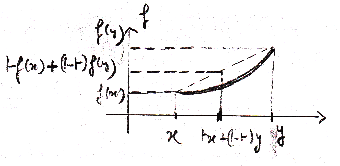
\includegraphics[scale=0.7]{7optim-dim1-convexe.png}
    \label{fig:7optim-dim1-convexe}
\end{figure}


\begin{fdef}
    $\deffonc{f}{\R^n}{\R}$ est strictement convexe si $\forall x,y \in \R^n$ tels
que $x \ne y, \forall t \in ]0,1[,$
    \[
        f(tx + (1-t)y) < tf(x) + (1-t) f(y)
    \]
\end{fdef}

\begin{ftheo}
    Si $\deffonc{f}{\R^n}{\R}$ est strictement convexe, il existe au plus un
    $x \in \R^n$ tel que $f(x) = \underset{y\in \R^n}{\Min f(y)}$.
\end{ftheo}

\begin{preuve}
    Supposons l'existene de deux minima en $x_1$ et $x_2$. Alors 
    \[
        f(tx_1 + (1-t)x_2) < tf(x_1) + (1-t) f(x_2) = f(x_1) = \underset{x \in \R^n}{\Min f(x)}
    \]

    On arrive alors à une contradiction.
\end{preuve}

\begin{remark}
    Ce théorème ne donne pas l'existence d'un minimum.

    Exemple :
\begin{figure}[h]
    \centering
    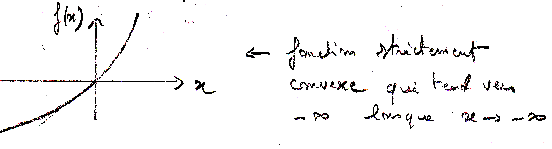
\includegraphics[scale=0.7]{7optim-min-str-cvx.png}
    \label{fig:7optim-min-str-cvx}
\end{figure}
\end{remark}

\begin{ftheo}
    Soit $\deffonc{f}{\R^n}{\R}$ strictement convexe et telle que $\underset{\norm{x} \longrightarrow +\infty}{\lim f(x)} = +\infty$. Alors il existe un unique $x \in \R^n$ tel que
    \[
        f(x) = \underset{y \in \R^n}{\Min f(y)}
    \]
\end{ftheo}

Nous allons maintenant relier les notions de point critique ($\nabla f(x) = 0$) et minimum
pour les fonctions convexes.

Le résultat suivant fournit une caractérisation utile de la convexité pour les fonctions
$\mathcal{C}^1$.

\begin{lemme}
    Soit $\deffonc{f}{\R^n}{\R}$ de classe $\mathcal{C}^1$.
    \begin{enumerate}[label=•]
        \item f est convexe si et seulement si 
            \[
                \forall x,y \in \R^n, \hspace{0.5cm} f(y) \geq f(x) + Df(x)(y-x)
            \]
        \item f est strictement convexe si et seulement si
            \[
                \forall x,y \in \R^n \text{ avec } x \ne y, \hspace{0.5cm} f(y) > f(x) + Df(x)(y-x)
            \]

            (résultat admis)
    \end{enumerate}
\end{lemme}

% Pas réussi à afficher l'image où il faut sans les vspaces ???
\vspace{0.1cm}
\subsubsection*{Interprétation en dimension 1 :}
\vspace{0.7cm}

\begin{figure}[h]
    \centering
    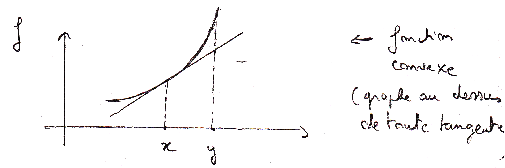
\includegraphics[scale=0.7]{7optim-cvx-tang.png}
    \label{fig:7optim-cvx-tang}
\end{figure}

\begin{ftheo}
    Soit $\deffonc{f}{\R^n}{\R}$ de classe $\mathcal{C}^1$ et convexe. Alors :
    \[
        f(x) = \underset{y \in \R^n}{\Min f(y)} \iff \nabla f(x) = 0
    \]
\end{ftheo}

\begin{preuve}
    \begin{enumerate}[label=•]
        \item ``$\implies$'' voir \S \textbf{1.1}
        \item ``$\Longleftarrow'' f(y) \geq f(x) + Df(x)\underbrace{(y-x)}_{= 0} \hspace{0.4cm} \forall y \in \R^n$
    \end{enumerate}
\end{preuve}

\begin{remark}
    On peut donc calculer numériquement les minima de fonctions convexes en recherchant
    les zéros de $x \mapsto \nabla f(x)$ (par exemple par la méthode de Newton).

    On admettra la caractérisation suivante de la convexité pour des fonctions $\Co^2$ :
\end{remark}

\begin{lemme}
    Soit $\deffonc{f}{\R^n}{\R}$ de classe $\Co^2$. Alors :

    \begin{enumerate}[label=•]
        \item $f$ est convexe $\iff \tpo{y} \; Hf(x) \; y \geq 0 \hspace{1cm} \forall x \in \R^n, \forall y \in \R^n$

        \item Si $Hf(x)$ est symétrique définie positive $\forall x \in \R^n$ alors $f$ est strictement convexe \footnotemark.
    \end{enumerate}
\end{lemme}\footnotetext{À vérifier, ce n'est pas lisible sur le kiosk}

\begin{remark}
    Pour $f(x) = \frac{x^4}{12}$ (strictement convexe), $H_f(x) = x^2$.

    $\implies H_f(0) = 0$ n'est pas symétrique définie positive.
\end{remark}

\subsubsection*{Application}
Soit $A \in M_n(\R)$ avec $A$ symétrique définie positive et $f(x)=\frac{1}{2} \tpo{x} \, A \, x - \tpo{b} \, x$

\[
    f(x) = \frac{1}{2} \sum_{i=1}^n \left( \sum_{j=1}^n a_{ij}x_j x_i \right) - \sum_{i=1}^n b_i x_i
\]

\[
    \Big( Hf \Big)_{(i,j)} = \frac{1}{2}(a_{ij} + a_{ji}) \implies
    Hf = \frac{1}{2}(A + \tpo{A}) = A \text{ (symétrique définie positive)}
\]

\[
    \implies f \text{ est strictement convexe.}
\]

De plus, $f(x) \longrightarrow +\infty$ quand $\norm{x} \longrightarrow +\infty$ car ($\lambda$ désigne
la plus petite valeur propre de $A$, qui est positive) :
\[
    f(x) \geq \frac{\lambda}{2} \norm{x}^2_2 - \norm{b}_2 \norm{x}_2 \longrightarrow +\infty \text{ quand } \norm{x}_2 \longrightarrow +\infty
\]

Donc il existe un unique $x \in \R^n \; / \; \MinI{\R^n} f = f(x)$.
Cette propriété est équivalente à $\nabla f(x) = 0$. 

\[
    \derpart{f}{x_i} = \frac{1}{2} \sum_{j=1}^n (a_{ij} + a_{ji})x_j - b_i
    \implies \nabla f(x) = \frac{1}{2}(A + \tpo{A})x - b
\]

Puisque $A$ est symétrique, $\nabla f(x) = Ax - b$. Donc :

\[
    Ax = b \iff f(x) = \MinI{\R^n} f \text{, avec } f(x) = \frac{1}{2}\tpo{x} \; A \; x - \tpo{b} x
\]

Cela permet de reformuler la résolution du système $Ax = b$ comme un problème
de minimisation.

\section{Quelques méthodes numériques pour l'optimisation sous contraintes :}

Nous abordons maintenant le calcul numérique d'un minimum de $\deffonc{f}{\R^n}{\R}$de classe $\Co^1$. On suppose que $\underset{\norm{x} \longrightarrow +\infty}{\lim} f(x) = +\infty$, de sorte que ce minimum existe.

Nous allons d'abord voir des \textbf{méthodes de gradient}, qui sont des
algorithmes itératifs utilisant uniquement $f$ et $\nabla f$.

L'exemple le plus simple d'une telle méthode est l'algorithme du
\underline{\textbf{gradient à pas constant}} :

\[
    \left\lbrace
    \begin{array}{cc}
        x_{k+1} = x_k - \rho \nabla f(x_k) & \hspace{1cm} \rho > 0 \text{ fixé} \\ [5pt]
        x_0 \in \R^n \text{ donné}
    \end{array}
    \right.
\]


Cette méthode est motivée par la propriété que $-\nabla f$ est orienté dans
le sens des valeurs de $f$ décroissantes.

On dit alors que $- \nabla f(x_k)$ est une \textbf{direction de descente} en $x_k$.

La méthode du gradient à pas constant est assez peu utilisée en pratique
car elle conduit facilement à des instabilités numériques. Par exemple,
pour $f(x) = x^4$ (fonction strictement convexe) on obtient $x_{k+1} = x_k(1-4 \rho x_k^2)$. Si $x_0^2 \geq \frac{1}{\rho}$, on montre par récurrence que
$|x_{k+1}| \geq 3 |x_k|$ (car $1-4\rho x_k^2 \leq - 3$) et donc $|x_k| \longrightarrow_{k\to +\infty} + \infty$.

Pour éviter ce type de phénomène, on peut considérer la \textbf{méthode de la
plus grande pente} (ou steepest descent method) dans laquelle $\rho$ est adapté
à chaque itération de manière \textbf{optimale} :

\[
    \begin{array}{cc}
        \left\lbrace
        \begin{array}{c}
            x_0 \in \R^n \text{ donné} \\[5pt]
            x_{k+1} = x_k - \rho_k \nabla f (x_k)
        \end{array}
        \right.
        & \hspace{1cm}
        f\left(x_k - \rho_k \nabla f(x_k)\right) = \MinI{\rho \geq 0} f \left(x_k - \rho \nabla f(x_k) \right)
    \end{array}
\]

À chaque étape de l'itération, il faut donc résoudre un problème de minimisation
en une dimension; plus précisément minimser la fonction $\deffonc{\phi}{\R^+}{\R}$ :
\[
    \rho \mapsto f(x_k - \rho \nabla f(x_k) ) := \phi (\rho)
\]
un minimum étant atteint en $\rho = \rho_k$ (le minimum existe sans être
nécessairement unique) puisque $\underset{\norm{x} \to +\infty}{\lim} f(x) = +\infty$.

\subsubsection*{Calcul de $\rho_k$ :}
Il y a plusieurs possibilités.
\begin{enumerate}[label=•]
    \item Méthode de Newton ou méthode de la sécante pour résoudre
        $\phi'(\rho) = 0$. Noter que c'est une condition nécessaire mais
        en général non suffisante pour obtenir un minimum.

        Cependant, si $f$ est convexe alors $\phi$ est aussi convexe (c'est
        la restriction de $f$ à une droite passant par $x_k$).

    Dans ce cas $\phi'(\rho) = 0 \iff \phi(\rho) = \MinI{y \in ]0,+\infty[}{\phi(y)}$

    \item Posons $a = 0$.
        
        On suppose $\deffonc{\phi}{[a,b]}{\R}$ unimodale, c.à.d. 
        \[
            \exists \rho^
        \in ]a,b[ \text{ tel que } \phi' < 0 \text{ sur } ]a,\rho^*[ \text{ et } \phi' > 0 
        \text{ sur } ]\rho^*, b[. 
        \]
        
        On pose $\delta = \dfrac{b-a}{4}, x_i = a + i\delta$.

        Selon la position relative des $f(x_i)$ ($i = 1,2,3$) on peut choisir
        $a' < b'$ tels que $f$ est unimodale sur $[a',b'] \subset [a,b]$ et
        $b' - a' = \frac{1}{2} (b - a)$. On recommence l'opération sur
        $[a',b']$ jusqu'à atteindre la précision souhaitée.


    \item \textbf{Cas particulier d'une fonction quadratique :}
        \[
            f(x) = \frac{1}{2} \tpo{x} \; A \; x - \tpo{b} \; x
        \]
    $A \in M_n(\R)$ symétrique définie positive, $b \in \R^n$.

    Notons $r_k = \nabla f(x_k) = A x_k - b \neq 0$ (sinon le min
    est déjà atteint !)

    $\phi'(\rho_k) = 0 \iff r_{k+1} . r_k = 0 \iff \underbrace{A x_k - \rho_k \: A \: r_k }_{Ax_{k+1}} - b) . r_k = 0$

    On obtient donc explicitement : 
    \[
        \rho_k = \frac{\norm{r_k}^2_2}{\tpo{r_k} \: A \: r_k}
    \]
    avec $\tpo{r_k} \: A \: r_k \neq 0$ puisque $A$ est symétrique définie
    positive.
\end{enumerate}

\begin{remark}
    En pratique le calcul de $p_k$ n'a pas besoin d'être réalisé avec
    une très grande précision.
\end{remark}

\noindent
\begin{tabular}{||c}
\begin{minipage}[c]{15cm}
        On peut montrer que la méthode de la plus grande pente converge pour toute
        condition initiale $x_0$ si $x$ est strictement convexe. La convergence
        est linéaire et peut donc être assez lente.
    \end{minipage}
\end{tabular}

\vspace{0.3cm}

\noindent
\begin{tabular}{||c}
    \begin{minipage}[c]{15cm}
        Pour avoir ue convergence plus rapide, on peut utiliser la méthode de
        Newton pour résoudre $\nabla f(x) = 0$. En particulier, si f est
        convexe on obtient ainsi forcément un minimum de $f$. Il existe par
        ailleurs des variantes moins coûteuses que Newton et efficaces, comme
        la méthode de Broyden.
    \end{minipage}
\end{tabular}

Une autre méthode beaucoup utilisée est la \textbf{méthode du gradient conjugué}.

Soit $\deffonc{f}{\R^n}{\R}$ de classe $\Co^2$, avec $f(x) \xrightarrow{\norm{x} \to +\infty} +\infty$
et $H_f(x)$ symétrique définie positive $\forall x \in \R^n$.

$f$ possède alors un minimum global strict $\overline{x} \in \R^n$. La méthode
du gradient conjugué utilise une direction de descente plus efficace que
$\nabla f(x_k)$, qui fait également appel à $\nabla f(x_{k-1})$. Nous allons
étudier cette méthode lorsque $f$ est une fonction quadratique mais elle
s'applique dans un cadre plus général.

\section{Méthode du gradient conjugé pour une fonction quadratique}

On considère $f(x) = \frac{1}{2} \tpo{x} \: A \: x - \tpo{b} \: x$ avec
$A \in M_n(\R)$ symétrique définie positive et $b \in \R^n$. Nous avons
vu que $\deffonc{f}{\R^n}{\R}$ admet un minimum global strict en $x = \overline{x}$ avec $A \overline{x} = b$.

La méthode du gradient conjugué définit une suite $(x_k)_{k\geq 0}$ qui
converge vers $\overline{x}$. Nous allons voir que la convergence se fait
en \textbf{un nombre fini d'itérations $\leq n$};  de ce point de vue,
la méthode du gradient conjugué est donc à classer parmi les méthodes
directes. Cependant, à cause des erreurs d'arrondis, cette propriété
n'est pas vérifiée en pratique (plus particulièrement pour de grands
systèmes) et la méthode est plutôt considérée comme itérative. On
contrôlera donc cet algorithme par un nombre maximal d'itérations et
par un test d'arrêt.

\subsection{Description de la méthode :}

\noindent
\begin{tabular}{||c}
    \begin{minipage}[c]{15cm}
        On notera par la suite $r_k = \nabla f(x_k) = A x_k - b$. Si
        $r_k = 0$ alors l'algorithme s'arrête ($x_k = ?$ illisible).
    \end{minipage}
\end{tabular}

\begin{enumerate}[label=\textit{\roman*})]
    \item \textbf{Initialisation :}
        On fixe $x_0 \in \R^n$.
        \begin{enumerate}[label=-]
            \item Si $x_0 = 0$ alors l'algorithme s'arrête car $x_0 = \overline{x}$.
            \item Si $x_0 \neq 0$, on calcule $x_1$ par la méthode de plus grande pente.

                On pose $\omega_0 = \nabla f(x_0)$. 
                
                $-\omega_0 =$ direction de pente pour calculer $x_1$.
                
                $x_1 = x_0 - \rho_0 \omega_0$, \hspace{0.5cm}
                $f(x_0 - \rho_0 \omega_0) = \MinI{\rho \geq 0} f(x_0 - \rho \omega_0)$

                \begin{remark}
                    Minimum explicite car minimse un polynôme de degré 2 en $\rho$.
                \end{remark}
        \end{enumerate}

    \item \textbf{Itération :}
        On suppose connus $x_k$ et $\omega_{k-1}$ ($-\omega_{k-1}$ est la direction de la pente
        utilisée pour calculer $x_k$).

        \begin{enumerate}[label=-]
            \item Si $r_k = 0$ alors l'algorithme s'arrête car $x_k = \overline{x}$.

            \item Si $r_k \neq 0$ : on pose
                \begin{align}
                    \omega_k & = r_k + \theta_k \omega_{k-1} \notag\\ 
                    \theta_k & = \frac{\tpo{r_k} (r_k - r_{k-1}}{\norm{r_{k-1}}_2^2}
                    \label{eq-optim:iteration}
                \end{align}
                ($-\omega_k =$ direction de la descente pour calculer $x_{k+1}$)
        \end{enumerate}

        $x_{k+1} = x_k - \rho_k \omega_k, \hspace{0.5cm} f(x_k - \rho_k \omega_k) = \MinI{\rho \geq 0} f(x_k - \rho \omega_k)$

        Dans le cas présent où $f$ est quadratique, la valeur de $\rho_k$ est
        connue explicitement (voir le lemme qui suit).
\end{enumerate}

Nous allons montrer les résultats suivants : (en patriculier, $r_k \neq 0$ implique
$\omega_k \neq 0$ puisque $r_k \perp \omega_{k-1}$


\begin{lemme}
    \begin{enumerate}[label=\textit{\roman*)}]
        \item $f(x_{k+1}) = \MinI{\theta \in \R} \MinI{\rho \geq 0} f \Big[ x_k - \rho(r_k + \theta \omega_{k-1} \Big]$

        \item $\tpo{r_k} w_{k-1} = 0, 
            \hspace{0.2cm} 
            \rho_k = \dfrac{\norm{r_k}^2_2}{\tpo{\omega_k} A \omega_k}$

        \item $\tpo{\omega_k} \: A \: \omega_{k-1} = 0 \hspace{0.5cm} (w_k \text{ et }
            \omega_{k-1} \text{ sont dits ``$A$-conjugés''})$
    \end{enumerate} 

    \label{lemme1}
\end{lemme}

\begin{lemme}
    $\tpo r_k \: r_{k-1} = 0$ et (\ref{eq-optim:iteration}) se transforme en :
    \begin{align}
        \theta_k = \frac{\norm{r_k}_2^2}{\norm{r_{k-1}}_2^2}
        \label{eq-optim:eqlemme}
    \end{align}
    \label{lemme2}
\end{lemme}

\begin{remark}
    Les formules (\ref{eq-optim:iteration}) et (\ref{eq-optim:eqlemme}) sont équivalentes pour
    une fonction $f$ quadratique. Pour $f$ plus générale, (\ref{eq-optim:iteration}) correspond
    à la méthode de Polak-Ribière et (\ref{eq-optim:eqlemme}) à celle de Fletcher-Reeves.
    La méthode du gradient conjugué dans le cas quadratique est dûe à Hestenes et
    Steifel (1952).
\end{remark}

\subsection{Preuve du lemme \ref{lemme1}}
Nous allons montrer successivement \textit{ii}), \textit{i}) et \textit{iii}).

Tout d'abord, puisque $f(x_{k-1} - \rho_{k-1} \omega_{k-1}) = \MinI{\rho \geq 0} f(x_{k-1} - \rho \omega_{k-1})$

On a $\nabla f(x_{k-1} - \rho_{k-1} \omega_{k-1}) - \omega_{k-1} = 0$, soit
$r_k \: \omega_{k-1} = 0 \implies \text{on a montré \textit{ii}) 1\up{ère} égalité.}$

Pour $\omega = r_k + \theta \omega_{k-1}$ on a (polnyôme du second degré en $\rho$.

\begin{align*}
    f(x_k - \rho \omega & = f(x_k) - \rho \nabla f(x_k) \: \omega + \frac{1}{2} \rho^2 \tpo \omega \: H_f(x_k) \: \omega \\
    & = f(x_k) - \rho \: r_k \: \omega + \frac{1}{2} \rho^2 \tpo \omega \: A \: \omega
\end{align*}

Puisque $r_k \: \omega_{k-1} = 0$, $r_k \: \omega$ est indépendant de $\theta$ et on obtient :
\begin{align}
    f(x_k - \rho \omega) = f(x_k) - \rho \norm{r_k}^2 + \frac{1}{2} \rho^2 \tpo \omega \: A \: \omega
    \label{eq-optim:4}
\end{align}

Le minimum de ce polynôme de degré 2 est atteint en :
\[
    \rho_{\theta} = \frac{\norm{r_k}^2_2}{\tpo \omega \: A \: \omega} \hspace{1cm}
    \text{2\up{ème} égalité de \textit{ii})}
\]

et vaut 
\[
    f(x_k - \rho_\theta \omega) = f(x_k) - \frac{1}{2} \frac{\norm{r_k}_2^4}{\tpo \omega \: A \: \omega}
\]

Pour minimiser $f(x_k - \rho_\theta \omega)$ suivant $\theta$ il faut minimiser 
$\tpo \omega \: A \: \omega$, c'est à dire $|\omega|$.
Il faut choisir pour cela $\omega = \omega_k$ tel que $\tpo \omega_k \: A \: \omega_{k-1} = 0$, ce qu'on notera $\omega_k \perp \omega_{k-1}$ :
\[
    < r_k + \theta \omega_{k-1}, r_k + \theta \omega_{k-1} = |r_k|^2 + 2 \theta <r_k, \omega_{k-1} >
    + \theta^2 |\omega_{k-1}|^2
\]

Minimum pour :
\begin{align}
    \theta = \theta_k = - \frac{<r_k, \omega_{k-1}>}{|\omega_{k-1}|^2}
    \label{l1:eq5}
\end{align}

Donc :
\begin{align}
    \omega_k = r_k - \omega_{k-1} \frac{<r_k,\omega_{k-1}>}{|w_{k-1}|^2}
    \label{l1:eq6}
\end{align}

D'où $\omega_k \perp \omega_{k-1}$. Afin de montrer le lemme \ref{lemme1}, il reste à
montrer que (\ref{l1:eq5}) correspond bien à (\ref{eq-optim:iteration}).
D'une part :
\begin{align}
    r_k - r_{k-1} = A \: (x_k - x_{k-1}) & = - \rho_{k-1} \: A \: \omega_{k-1} \hspace{0.5cm}\text{ donc :} \notag \\
    \tpo r_k (r_k - r_{k-1}) & = - \rho_{k-1} <r_k,\omega_{k-1}>
    \label{l1:eq7}
\end{align}

D'autre part :
\begin{align*}
    |\omega_{k-1}|^2 & = (A \omega_{k-1}, \omega_{k-1}) = -\frac{1}{\rho_{k-1}}(A (x_k - x_{k-1}), \omega_{k-1}) \\
    & = -\frac{1}{\rho_{k-1}}(r_k - r_{k-1} , \omega_{k-1}) \\
    & = \frac{1}{\rho_{k-1}}(r_{k-1}, \omega_{k-1}) \hspace{2cm} \text{(car $(r_k,\omega_{k-1}) = 0$)}\\
    & = \frac{1}{\rho_{k-1}}(r_{k-1},r_{k-1}- \theta_{k-1}\omega_{k-2}) \\
    & = \frac{1}{\rho_{k-1}}\norm{r_k}^2 \hspace{2cm} \text{(car $(r_{k-1}, \omega_{k-2}) = 0$)}
\end{align*}

Donc :
\begin{align}
    \norm{r_k}^2 = \rho_{k-1} |\omega_{k-1}|^2
    \label{l1:eq8}
\end{align}

Avec (\ref{l1:eq5}), (\ref{l1:eq7}) et (\ref{l1:eq8}) on obtient donc :
\[
    \frac{\tpo r_k (r_k - r_{k-1}}{\norm{r_{k-1}^2}}  - \frac{<r_k,\omega_{k-1}>}{|\omega_{k-1}|^2} = \theta_k
\]

On obtient donc la formule (\ref{eq-optim:eqlemme}) plus simple pour le calcul de $\theta_k$.

\subsection{Convergence de la méthode du gradient conjugué et preuve du \ref{lemme2}}

Supposons $r_k \ne 0$ pour $k = 0,\dots,n-1$ (si $r_k$ s'annule l'algorithme converge). Cela implique
$\rho_k \ne 0$ pour $k=0,\dots,n-1$.

\begin{lemme}
    Pour tout $k=1,\dots,n$ on a :
    \[
        \begin{array}{cc}
            (P_k) &
            \left\lbrace
            \begin{array}{cc}
                r_k \: \omega_q = 0 & \text{pour $q = 0,\dots,k-1$} \\
                \tpo \omega_k \: A \omega_q = 0 & \text{pour $q = 0,\dots,k-1$} \\
                r_k \: r_q = 0 & \text{pour $q = 0,\dots,k-1$} \\
            \end{array}
            \right.
        \end{array}
    \]
    \label{lemme3}
\end{lemme}

\begin{preuve}
    Par récurrence. On considère les produits scalaires 
    \[
        \left\lbrace
        \begin{array}{ccc}
            (x,y) & = & \tpo xy = x.y \\
            & \text{et} & \\
            <x,y> \: & = & \tpo x \: A \: y
        \end{array}
        \right.
    \]

    \begin{enumerate}[label=•]
        \item $P_1$ est vraie : $r_1 \: r_0 = r_1 \: \omega_0 = 0$ (condition d'optimalité de $\rho_0$)

            \[
                < \omega_1 , \omega_0 > = 0 \hspace{1cm} \text{d'après le lemme 1}
            \]

        \item Supposons $P_k$ vraie et montrons $P_{k+1} (k \leq n-1)$. On a :

            \[
                r_{k+1}.\omega_k = 0 \hspace{1cm} \text{(condition d'optimalité de $\rho_k$)}
            \]

            \begin{align*}
                r_{k+1}.\omega_q & = (Ax_{k+1} - b, \omega_q) = \left(A(x_{k+1} - x_k) + Ax_k - b, \omega_q \right) \\
                & = - \rho_k <\omega_k,\omega_q> + r_k . \omega_q \\
                & = 0 \hspace{0.5cm} \text{pour $q=0,..,k-1$ (hyp de récurrence $P_k$)}
            \end{align*}

            Donc $r_{k+1}.\omega_q = 0$ pour $q=0,..,k$.

            Par ailleurs, $r_{k+1}.r_q = r_{k+1}.(\omega_q - \theta_q \omega_{q-1})$ \hspace{0.3cm} (avec $\theta_0 := 0$ car $r_0 = \omega_0$)

            \vspace{0.4cm}
            Donc $r_{k+1}.r_q = 0$ pour $q=0,..,k$

            \vspace{0.4cm}
            Ensuite $<\omega_{k+1},\omega_k> = 0$ d'après le lemme \ref{lemme1}, et pour
            $q=0,\dots,k-1$ :
            \[
                <\omega_{k+1},\omega_q> = <r_{k+1},\omega_q> + \theta_{k+1} <\omega_k,\omega_q> = <r_{k+1},\omega_q>
            \]
            (par l'hypothèse de récurrence $P_k$)

            \vspace{0.4cm}
            $\rho_{q+1} - r_q = A(x_{q+1}-x_q) = - \rho_q \; A \; \omega_q$ amène alors :
            \begin{align*}
                <\omega_{k+1},\omega_q> & = <r_{k+1}, \omega_q> = \frac{1}{\rho_q}(r_{k+1},-r_{q+1}+r_q) \\
                & = 0
            \end{align*}
            car $0 \leq q \leq k-1$ et $(r_{k+1},r_p) = 0$ pour $p = 0,\dots,k$

            Cela prouve $P_k$ par récurrence.
    \end{enumerate}
\end{preuve}

En conclusion, la famille $(\omega_0, \dots, \omega_{n-1})$ est libre car les $\omega_i$ sont
deux à deux orthogonaux pour le produit scalaire $<x,y> = \tpo x \; A \; y$. C'est donc une
base de $\R^n$. Puisque $r_n$ est orthogonal à $\omega_0, \dots, \omega_{n-1}$, on a donc
$r_n=0$. Nous avons donc montré que $A \, x_n = b$, i.e. $x_n=??$

\begin{ftheo}
    Soit $A \in M_n(\R)$ symétrique définie positive, $b \in \R^n$ et ${f(x) = \frac{1}{2} \tpo x \: A \: x - \tpo b \: x}$.
    Alors l'algorithme du gradient conjugué définit une suite $(x_k)_{k=0,\dots,p}$ avec
    $p \leq n$ et $A \: x_p = b$. On a $f(x_p) = \MinI{x \in \R^n} f(x)$.
\end{ftheo}

\begin{remark}
    Le cas $p<n$ est exceptionnel.
\end{remark}

Enfin, nous avons montré dans le lemme \ref{lemme3} que $r_k.r_{k-1}=0$, ce qui prouve le lemme
\ref{lemme2}.


\chapter{Rappels}

\section{Matrice Jacobienne}

La matrice jacobienne est la matrice des dérivées partielles du premier ordre d'une fonction vectorielle.

Soit F une fonction d'un ouvert de $\mathbb{R}^n$ à valeurs dans $\mathbb{R}^m$. Une telle fonction est définie par ses m fonctions composantes à valeurs réelles :

\begin{equation*}
F : \begin{pmatrix}x_1\\\vdots\\x_n\end{pmatrix} \longmapsto \begin{pmatrix}
f_1(x_1,\dots,x_n)\\
\vdots\\
f_m(x_1,\dots,x_n)\end{pmatrix}
\end{equation*}
\\

Les dérivées partielles de ces fonctions en un point M, si elles existent, peuvent être rangées dans une matrice à m lignes et n colonnes, appelée matrice jacobienne de F :

\begin{equation*}
J_F\left(M\right)=
\begin{pmatrix} 
\dfrac{\partial f_1}{\partial x_1} & \cdots & \dfrac{\partial f_1}{\partial x_n} \\
\vdots & \ddots & \vdots \\
\dfrac{\partial f_m}{\partial x_1} & \cdots & \dfrac{\partial f_m}{\partial x_n}
\end{pmatrix}
\end{equation*}
\\

On suppose maintenant que $m = n$. On appelle jacobien de $f$ le déterminant de sa matrice jacobienne noté : $\det( J_F )$.



\section{Valeurs propres d'une matrice}

Les valeurs propres $\lambda$ et le vecteur propre $x$ d'une matrice A respectent :
\begin{equation*}
(A - \lambda I) \, x = 0
\end{equation*}

On les calcule en résolvant l'équation :
\begin{equation*}
\det(A - \lambda I) = 0
\end{equation*}


\section{Calcul du déterminant}

Pour toute matrice carrée de la forme : 

\begin{equation*}
A = \begin{pmatrix} a_{11} & \cdots & a_{1n} \\ \vdots & \ddots & \vdots \\ a_{n1} & \cdots & a_{nn} \end{pmatrix}
\end{equation*}

Le déterminant est :

\begin{equation*}
\det(A) = \begin{vmatrix} a_{11} & \cdots & a_{1n} \\ \vdots & \ddots & \vdots \\ a_{n1} & \cdots & a_{nn} \end{vmatrix}
\end{equation*}


\subsection{Dimension 2}

\begin{equation*}
\begin{vmatrix}a&b\\c&d\end{vmatrix} = \, ad - bc
\end{equation*}


\subsection{Dimension 3}

\begin{equation*}
\begin{vmatrix}a&b&c\\d&e&f\\g&h&i\end{vmatrix} =
\begin{array}{cc}
\, \, \, \, \, \, \, a \, e \, i + b \, f \, g + c \, d \, h\\
- \, g \, e \, c - h \, f \, a - i \, d \, b
\end{array}
% \, \, \, \, \, \, \, a \, e \, i + b \, f \, g + c \, d \, h\\
% &\, \, \, \, \, \, \, \, - g \, e \, c - h \, f \, a - i \, d \, b
% &\, \, \, \, \, \, \, \, - (g\cdot e\cdot c + h\cdot f\cdot a + i\cdot d\cdot b)
\end{equation*}


\subsection{Dimension n}

Pour tout i et j, on note $A_{ij}$ la matrice obtenue en enlevant à A sa i-ième ligne et sa j-ième colonne :

\begin{equation*}
A_{ij}=\begin{pmatrix}a_{1,1} & \dots & a_{1,j-1}& a_{1,j+1}& \dots & a_{1,n} \\\vdots & & \vdots &  \vdots& &\vdots\\
a_{i-1,1} & \dots & a_{i-1,j-1}& a_{i-1,j+1}& \dots & a_{i-1,n} \\
a_{i+1,1} & \dots & a_{i+1,j-1}& a_{i+1,j+1}& \dots & a_{i+1,n} \\
\vdots & & \vdots & \vdots &&\vdots\\
a_{n,1} & \dots & a_{n,j-1}& a_{n,j+1}& \dots & a_{n,n}\end{pmatrix} 
\end{equation*}


On peut alors développer le calcul du déterminant de A suivant une ligne ou une colonne.
\\

Développement suivant la ligne $i$ :
\begin{equation*}
\large{\fbox{$\det(A)=\sum \limits_{j=1}^{n} a_{ij} \cdot (-1)^{i+j} \cdot \det(A_{ij})$}}
\end{equation*}

Le terme $(-1)^{i+j} \cdot \det(A_{i,j})$ est appelé cofacteur du terme $a_{ij}$.



\section{Inverse d'une matrice}

Une matrice carrée $M$ est inversible si et seulement si son déterminant est non nul :
\begin{equation*}
\exists M^{-1} \iff \det(M) \ne 0
\end{equation*}



\section{Matrice définie positive}

Une matrice $M$ est dite définie positive si toutes ses valeurs propres sont strictement positives, c'est-à-dire :
\begin{equation*}
\mathrm{Sp}(M) \subset\,\, ]0, +\infty[
\end{equation*}


\section{Matrice symétrique}

Une matrice $M$ est dite symétrique si $\forall (i, j), m_{ij} = m_{ji}$.


\section{Matrice symétrique définie positive}

Une matrice $M$ est dite symétrique définie positive (SDP) si elle est définie positive et symétrique.





\end{document}
